\documentclass[manuscript,anonymous,review]{acmart}
% Anonymous double-blind review submission mode, per JDIQ_GUIDELINE_SUMMARY.md Sec.4-5.
% Do NOT alter margins, spacing, or font definitions in this file or via \geometry etc.
% Upon acceptance: remove the "manuscript,anonymous,review" options and submit to ACM TAPS.
\usepackage{amsmath}
\usepackage{placeins}
% NOTE: amssymb is NOT loaded here -- acmart already loads it internally, and
% an explicit \usepackage{amssymb} clashes on \Bbbk ("already defined").
% Discovered and fixed during this pass's compile-and-fix step.

\AtBeginDocument{%
  \providecommand\BibTeX{{\normalfont B\kern-0.5em{\scshape i\kern-0.25em b}\kern-0.25em T\kern-0.1667em\lower0.7ex\hbox{E}\kern-0.125emX}}}

% ---------------------------------------------------------------------------
% CCS concepts (required for articles > 2 pages, JDIQ_GUIDELINE_SUMMARY.md Sec.4)
% ---------------------------------------------------------------------------
\begin{CCSXML}
<ccs2012>
   <concept>
       <concept_id>10002951.10003317.10003347.10003348</concept_id>
       <concept_desc>Information systems~Data cleaning</concept_desc>
       <concept_significance>500</concept_significance>
       </concept>
   <concept>
       <concept_id>10002951.10003317.10003347</concept_id>
       <concept_desc>Information systems~Data quality</concept_desc>
       <concept_significance>500</concept_significance>
       </concept>
   <concept>
       <concept_id>10002951.10003227.10003236</concept_id>
       <concept_desc>Information systems~Retrieval models and ranking</concept_desc>
       <concept_significance>500</concept_significance>
       </concept>
   <concept>
       <concept_id>10002951.10003317.10003359</concept_id>
       <concept_desc>Information systems~Data cleaning</concept_desc>
       <concept_significance>300</concept_significance>
       </concept>
</ccs2012>
\end{CCSXML}

\ccsdesc[500]{Information systems~Data cleaning}
\ccsdesc[500]{Information systems~Data quality}
\ccsdesc[500]{Information systems~Retrieval models and ranking}
% TODO(manuscript-authors): Verify final CCS concept IDs against the ACM CCS
% generator (https://dl.acm.org/ccs) before submission; ids above are drawn
% from papers/JDIQ_2026/JDIQ_GUIDELINE_SUMMARY.md Sec.4 and MANUSCRIPT_OUTLINE.md
% front-matter, not independently re-verified against the live CCS tool here.

\keywords{preference graphs, data quality, structural inconsistency, rank aggregation,
  feedback arc set repair, retrieval evaluation, benchmark curation}
% Keywords per MANUSCRIPT_OUTLINE.md front matter (Title page section).

% ---------------------------------------------------------------------------
% Title / authors
% ---------------------------------------------------------------------------
% TODO(manuscript-authors): provisional title; see PROJECT_STATUS.md / CANONICAL_PAPER_STORY.md
% for two alternative titles under consideration.
\title{When Does Repairing Preference-Graph Inconsistency Improve Retrieval Quality?
  A Multi-Benchmark Data Quality Study}

% Anonymous submission: author block intentionally omitted/placeholder per
% acmart's anonymous,review mode and JDIQ_GUIDELINE_SUMMARY.md Sec.5 anonymization checklist.
\author{Anonymous Author(s)}
\affiliation{%
  \institution{Institution redacted for review}
  \country{}
}

\begin{document}

% ---------------------------------------------------------------------------
% Abstract
% ---------------------------------------------------------------------------
\begin{abstract}
Retrieval systems that combine multiple ranking signals often represent
disagreement between them as a directed preference graph, where an edge
records evidence that one document should rank above another. When signals
disagree enough, this graph can contain cycles, so no single ordering can
satisfy every recorded preference --- a structural data-quality defect in a
derived artifact. A standard remedy repairs the graph by removing a
minimum-weight set of cycle-inducing edges before extracting a final
ranking. This paper asks whether that structural repair also improves the
quality of the resulting ranking, measured by a standard graded-relevance
retrieval metric. Across four public retrieval benchmarks and three
graph-construction regimes, we find that vote construction, not repair, is
the dominant driver of graph inconsistency, and that repair reliably
improves graph-level consistency whenever inconsistency is present. This
structural improvement, however, translates into a measurable
ranking-quality gain in only one of twelve dataset-and-regime combinations
tested, and simple score-fusion baselines that never inspect graph structure
remain competitive with, or better than, every graph-repair method
evaluated. A manual failure-class analysis identifies why repair is usually
inactive, occasionally neutral, and rarely harmful, offering practical
guidance on when this intervention is worth applying. We release a
companion benchmark packaging the underlying graphs, repair outcomes, and
diagnostic labels to support further research on preference-graph data
quality. We make no claim that structural repair is a generally superior
retrieval strategy; the evidence instead supports treating structural
consistency and retrieval quality as related but distinct measures that
must be evaluated separately.
\end{abstract}

\maketitle

% =============================================================================
\section{Introduction}
\label{sec:introduction}
% Full first-draft prose below. See INTRODUCTION_EVIDENCE_MAP.md for a
% sentence-by-sentence trace of every empirical claim to its canonical source,
% and REVIEWER_CONCERN_COVERAGE.md for how this section answers each of the
% ten prior-reviewer concerns.

Modern retrieval pipelines rarely rely on a single ranking signal. It is
increasingly common to combine sparse retrievers, dense retrievers,
cross-encoders, and large language models operating in pointwise, pairwise, or
listwise comparison modes, and to treat their outputs as evidence to be
aggregated rather than as a final answer~\cite{liu2011learning,burges2005learning,sun-etal-2023-chatgpt,qin-etal-2024-large}.
A natural way to combine such heterogeneous signals is to represent them as a
weighted, query-specific preference graph: a directed edge from document $u$ to
document $v$ records evidence that $u$ should be ranked ahead of $v$, and
edge weight records the strength of that evidence~\cite{dwork2001rank,ailon2008aggregating,negahban2017rankcentrality}.
This representation is attractive precisely because it keeps disagreement
visible instead of collapsing it immediately into a single scalar score. But
that same property is also its central liability from a data-quality
standpoint: once preferences from multiple rankers are aggregated into a
graph, the graph can contain directed cycles, meaning the aggregated evidence
cannot be represented by any single, globally consistent ordering.

We treat this cyclicity as what it is: a structural data-quality defect in a
\emph{derived} data artifact. The preference graph is not raw data collected
from the world; it is manufactured by a specific aggregation procedure applied
to upstream ranker scores, and its consistency properties are a direct
consequence of that procedure. Viewed this way, a cyclic preference graph is
analogous to other well-studied information-quality problems in derived
data---contradictory records, non-integrable schemas, or inconsistent
provenance chains---in that the defect is measurable, its severity depends on
how the data was constructed, and it invites a natural remediation step.
Feedback-arc-set (FAS) repair is exactly such a remediation step for preference
graphs: it removes the minimum-weight set of edges needed to make the graph
acyclic, producing a graph that is, by construction, more internally
consistent~\cite{ailon2008aggregating,kenyon2007fewerrors}.

The unresolved question is whether this kind of structural repair is worth
performing from the standpoint of the information a retrieval system ultimately
delivers to a user. Structural consistency and downstream retrieval quality
are related but conceptually distinct notions of ``quality.'' A repaired graph
is more internally consistent by the metric that defines the repair, but
consistency is not the same property that a ranked-retrieval metric such as
normalized discounted cumulative gain (nDCG) measures. It is possible for a
repair intervention to measurably improve
graph-level consistency while leaving the final ranked list unchanged, or even
making it worse, if the edges it removes happen to be uninformative or
misleading with respect to the relevance judgments a retrieval system is
ultimately evaluated against. Prior work on rank aggregation and feedback-arc-set
methods has largely emphasized the algorithmic and structural side of this
problem---how to find a good repair, and how to bound its
approximation quality relative to a graph-internal objective~\cite{dwork2001rank,ailon2008aggregating,kenyon2007fewerrors,fagin2003comparing}---without
systematically testing whether the resulting structural improvement transfers
to the retrieval-quality outcome that end users experience. This leaves a gap:
it is not enough to show that a repair procedure exists and reduces a
structural inconsistency score; a data-quality account of preference-graph
repair also has to characterize when, and how reliably, that structural
improvement translates into better ranked output, and to say plainly when it
does not.

This paper closes that gap empirically. We study preference-graph
inconsistency as a measurable data-quality dimension and evaluate feedback-arc-set
repair as a candidate data-quality improvement technique, across four public
retrieval benchmarks (SciDocs, FiQA, HotpotQA, and BRIGHT) and three
vote-extraction regimes that construct preference graphs from the same
underlying ranker scores under different retention rules for directional
evidence~\cite{cohan2020scidocs,maia2018fiqa,yang2018hotpotqa,su2024bright}. This
design lets us separate three choices that are often bundled together in
reranking pipelines but that have distinct consequences: how permissively
pairwise votes are retained during graph construction, whether the resulting
graph is repaired before scoring, and which graph-scoring rule is used to turn
the (repaired or unrepaired) graph into a ranking. Because vote-extraction
regime alone determines whether a graph has any cyclic structure for repair to
act on, we report every structural and retrieval outcome broken out by regime
rather than pooled, so that a null result in a near-acyclic regime is not
mistaken for a failure of the repair procedure itself.

Two results follow from this design, and both are load-bearing for the paper's
contribution rather than incidental. First, vote-extraction regime, not the
repair step, is the dominant driver of preference-graph inconsistency: a
conservative, majority-style regime keeps graphs almost entirely acyclic on
every dataset we test, while a permissive regime that retains every
ranker-supported directional vote produces substantially cyclic graphs with
much larger strongly connected components. Second, and centrally, we find
that structural improvement from repair and downstream retrieval improvement
are decoupled in the large majority of the conditions we test. When the
underlying graph is already near-acyclic, repair is retrieval-inactive by
construction, because there is negligible conflicting edge weight for it to
remove. Even in the one regime where graphs are substantially cyclic, the
retrieval effect of repair is heterogeneous across datasets and, in three of
four cases, statistically indistinguishable from no effect once bootstrap
uncertainty is taken into account; a single dataset shows a reliable positive
effect, and it is not the dataset with the most severe structural
inconsistency. We treat these null and mixed outcomes as part of the
contribution, not as a shortfall to be explained away: identifying the
conditions under which a data-quality intervention does \emph{not} transfer to
task-level utility is itself the actionable finding a practitioner needs
before deciding whether to invest in graph repair for a given pipeline.

We are careful about what this study does and does not claim, in part because
an earlier version of this analysis was reviewed and found wanting on several
specific grounds that we address directly in the study design rather than in
prose alone. The evaluation is not built solely on the narrow BM25/TF-IDF/MiniLM
ranker family; we additionally test a bounded, cross-dataset sample of
real large-language-model pairwise, pointwise, and listwise judgments to check
whether the same regime-conditional pattern persists under genuine LLM
preferences, while being explicit that this LLM evidence remains small in
scale and is reported as a supporting check rather than a confirmatory result
in its own right. We do not rely on a single repair algorithm in isolation:
the greedy feedback-arc-set heuristic used in the main experiments is compared
against stronger exact and near-exact repair variants, which improve the
graph-internal structural objective further but do not change the retrieval
conclusion. We do not restrict the comparison to the repaired-versus-unrepaired
pair alone; we additionally evaluate the repaired hybrid rankings against a
broad grid of fixed aggregation baselines, including reciprocal rank fusion
(RRF) and CombSUM, to test whether graph repair is competitive with much simpler
alternatives once retrieval quality, rather than structural consistency, is
the criterion. Because the hybrid rankings we evaluate combine a graph-derived
component with a prior score vector by fusion, we also examine directly whether
that fusion step itself can mask a graph-level change, so that a null retrieval
result is not silently misattributed to repair being unhelpful when it may
instead reflect the fusion weighting absorbing the repair signal. Finally,
where a graph-based diagnostic such as backward-edge weight is computed against
the same relevance judgments used for retrieval evaluation, we flag that
circularity explicitly rather than presenting it as independent corroboration.

Framed this way, the contribution of this paper is diagnostic and curatorial
rather than algorithmic. We do not propose a new ranking algorithm, and we do
not claim that feedback-arc-set repair is a generally superior reranking
strategy; the evidence does not support that claim, and we say so directly.
Instead, we contribute: (1) a systematic, regime-stratified measurement of
preference-graph structural inconsistency across four benchmarks and 1{,}006
query$\times$regime evaluation records (Table~\ref{tab:dataset-stats}); (2) a
bootstrap-quantified account of when feedback-arc-set repair does and does
not change downstream retrieval
quality, including the single regime in which it reliably does; (3) a
six-class failure taxonomy that explains \emph{why} repair is retrieval-inactive,
neutral, or harmful in specific, interpretable terms, rather than reporting
only aggregate null results; (4) a pooled comparison showing that simple,
fixed aggregation baselines are competitive with or superior to repaired
graph-hybrid rankings, which bears directly on whether structural repair is a
good investment relative to simpler alternatives; and (5) the release of a
curated companion benchmark resource, the Consistency-Aware Reranking
Benchmark (CARB), that packages the graph-theoretic features, repair
outcomes, and ranking scores underlying these findings for reuse in
future data-quality research on preference graphs. Together, these
contributions position preference-graph consistency as a data-quality problem
to be measured and diagnosed on its own terms, with retrieval effectiveness
treated as a separate, empirically evaluated outcome rather than an assumed
consequence of structural repair.

The remainder of the paper is organized as follows. Section~2 (Background)
positions this study relative to data-quality frameworks, rank aggregation and
preference modeling, and rank fusion. Section~3 (Methodology) formalizes
preference graphs, the structural data-quality metrics we measure, the
feedback-arc-set repair operator, and the ranking-extraction rules applied
before and after repair. Section~4 (Experimental Setup) describes the
four-dataset protocol, vote-extraction regimes, baselines, and evaluation
methodology, including the bootstrap procedure used throughout. Sections~5--7
report structural results, the repaired-versus-unrepaired retrieval comparison
with bootstrap confidence intervals, and the failure taxonomy, respectively.
Section~8 reports the bounded real-LLM validation, and Section~9 summarizes
runtime and memory implications. Section~10 introduces the CARB benchmark.
Section~11 discusses the findings, Section~12 states limitations, and
Section~13 concludes; a final section states data and reproducibility
availability.

% =============================================================================
\section{Background}
\label{sec:background}
% Written from scratch for this pass (not copied from the IJCS source); see
% IJCS_REUSE_AUDIT.md Sec.3.1 for the verified notation this section reuses.
% TODO(manuscript-authors): a full literature-positioning Related Work section
% (comparison table against Dwork/Ailon-Charikar-Newman/prior MWFAS work, per
% docs/LITERATURE_ALIGNMENT.md) remains future work; this section intentionally
% stays a compact background rather than a survey, per this pass's scope.

Preference-based ranking systems are usually built from more than one signal
of relative quality: multiple retrievers, multiple cross-encoders, or multiple
large-language-model judgments operating over the same candidate set. A
convenient way to represent such evidence, rather than collapsing it
immediately into a single scalar score, is a directed \emph{preference graph}.

\textbf{Preference graphs.} For a query $q$ with candidate documents
$D_q=\{d_1,\dots,d_n\}$, a preference graph is a weighted directed graph
$G_q=(V_q,E_q,w_q)$ with $V_q=D_q$. A directed edge $(u,v)\in E_q$ records
evidence for the pairwise preference $u \succ v$ (``$u$ should be ranked ahead
of $v$''), and $w_q(u,v)>0$ is the strength of that evidence, aggregated from
one or more underlying rankers. This representation is standard in rank
aggregation and pairwise-comparison ranking~\cite{dwork2001rank,ailon2008aggregating,negahban2017rankcentrality}:
it keeps disagreement between rankers visible as graph structure instead of
discarding it during fusion.

\textbf{Structural inconsistency.} A ranking is a total order on $V_q$. If
$G_q$ is acyclic, at least one total order exists that agrees with every edge
direction (any topological order of $G_q$). If $G_q$ contains a directed
cycle---a sequence of edges $u_1 \to u_2 \to \cdots \to u_k \to u_1$---no
total order can respect every edge in the cycle simultaneously: some pairwise
preference in the aggregated evidence must be violated by any ranking. This
is not a pathological edge case particular to any one aggregation rule. Even
when every individual ranker's own preferences are transitive, aggregating
several rankers' preferences over the same pair can still produce a cycle
whenever different rankers disagree about the direction of a pair and both
directions are retained in the merged graph---the same structural phenomenon
that produces majority cycles in social-choice
aggregation~\cite{dwork2001rank,ailon2008aggregating}. We call a query's
preference graph \emph{structurally inconsistent} when it is cyclic, and we
treat cyclicity, together with related graph properties defined in
Section~\ref{sec:methodology} (largest strongly connected component size,
backward-edge weight, pairwise inconsistency count), as measurable
\emph{structural data-quality} dimensions of the graph: they describe a
property of the derived artifact $G_q$ itself, independent of any downstream
use.

\textbf{Repair via feedback arc sets.} Because $G_q$ is a \emph{derived} data
product---manufactured from upstream ranker scores by a specific
construction procedure, not observed directly---its inconsistency can in
principle be reduced by removing a subset of edges. The \emph{feedback arc
set} (FAS) problem asks for the minimum-weight subset of edges whose removal
leaves an acyclic graph; equivalently, it asks for a total order on $V_q$ that
minimizes the total weight of preference edges it violates. This
formulation of ranking as weighted feedback-arc-set minimization is classical
in rank aggregation~\cite{ailon2008aggregating,kenyon2007fewerrors}, is
NP-hard in general~\cite{ailon2008aggregating}, and is the formal basis for
the repair operator we use (Section~\ref{sec:methodology}): repair is, by
this definition, an operation on the graph's internal edge-violation
objective, not an operation defined with reference to any external relevance
judgment.

\textbf{Why structural repair need not improve retrieval quality.} This last
point is the crux of the data-quality question this paper studies. A repaired
graph $\widetilde G_q$ is, by construction, weakly more consistent than $G_q$
under the objective FAS minimizes---removing edges cannot increase the total
violated weight. But nothing in that guarantee constrains what happens to a
\emph{downstream} ranking metric such as nDCG, which is computed against
relevance judgments the FAS objective never sees. The two notions of
``quality'' are formally independent: one is an intrinsic property of the
graph relative to its own edge weights; the other is an extrinsic property of
a ranking relative to a separate ground-truth signal. Whether an edge removed
by repair happened to be aligned with, orthogonal to, or contrary to the
relevance judgments is not something the FAS objective is designed to know.
Prior work on feedback-arc-set-based ranking has focused on the algorithmic
side of this problem---finding a good or provably-bounded
repair~\cite{dwork2001rank,ailon2008aggregating,kenyon2007fewerrors,fagin2003comparing}---which
is a necessary but not sufficient condition for the repair to matter to a
retrieval system's users. Sections~\ref{sec:methodology}
and~\ref{sec:experimental-setup} make this distinction operational: we report
structural metrics and retrieval metrics as two separate families of
measurement on the same graphs, precisely so that the relationship between
them is an empirical question rather than an assumption.

% =============================================================================
\section{Methodology}
\label{sec:methodology}
% Written from scratch and verified line-by-line against the implementation in
% src/consistency_ranker/{pairwise_prefs,graph_construction,greedy_fas,
% exact_fas,mwfas_solver,evaluation}.py and scripts/{build_votes_file,
% postprocess_votes_drop_mutual_pairs,run_real_experiment,
% run_publication_vote_suite}.py during this pass. Formulas below match the
% code, not the IJCS manuscript's equations, wherever the two differ (see
% inline notes).

This section defines the preference-graph construction procedure, the
structural data-quality metrics computed on it, the feedback-arc-set repair
operator, and the ranking-extraction rules applied to a graph before and
after repair. We keep these four stages notationally and conceptually
distinct throughout, because conflating them is a recurring source of
ambiguity in prior discussions of ``graph repair for reranking'': repair
changes which edges a graph contains; extraction turns a (fixed) set of edges
into a ranking. The same extraction rule is applied to both the unrepaired
and the repaired graph, so any difference in the resulting ranking is
attributable to repair and not to a change in the extraction rule itself.
Table~\ref{tab:notation} summarizes notation used in this section and
Section~\ref{sec:experimental-setup}.

\begin{table}[t]
  \caption{Notation used in Sections~\ref{sec:methodology}
    and~\ref{sec:experimental-setup}.}
  \label{tab:notation}
  \begin{tabular}{cl}
    \toprule
    Symbol & Meaning \\
    \midrule
    $q$, $D_q$ & Query and its candidate document set \\
    $G_q=(V_q,E_q,w_q)$ & Preference graph for query $q$ ($V_q = D_q$) \\
    $\widetilde G_q$ & Repaired (acyclic) preference graph \\
    $u \succ v$ & Pairwise preference: $u$ ranked ahead of $v$ \\
    $r$ & Vote-extraction regime, $r\in\{\texttt{ms2},\texttt{ms1},\texttt{ms1\_drop\_mutual}\}$ \\
    $F$ & A feedback arc set (edge subset removed by repair) \\
    $\deg^+(u),\deg^-(u)$ & Out-degree, in-degree of node $u$ in a graph \\
    $s_{\mathrm{cop}}, s_{\mathrm{bal}}$ & Copeland score, weighted balance score \\
    $\hat{s}(\cdot)$ & Min--max normalization of a score vector to $[0,1]$ \\
    $\alpha$ & Hybrid mixing weight for the graph-derived component \\
    $\pi$ & A ranking (permutation) of $V_q$ \\
    $\mathrm{BEW}(\pi,G)$ & Backward-edge weight of $\pi$ relative to graph $G$ \\
    $\mathrm{PIC}(\pi,G)$ & Pairwise inconsistency count (unweighted analogue) \\
    $k$ & nDCG cutoff \\
    \bottomrule
  \end{tabular}
\end{table}

\begin{figure}[t]
  \centering
  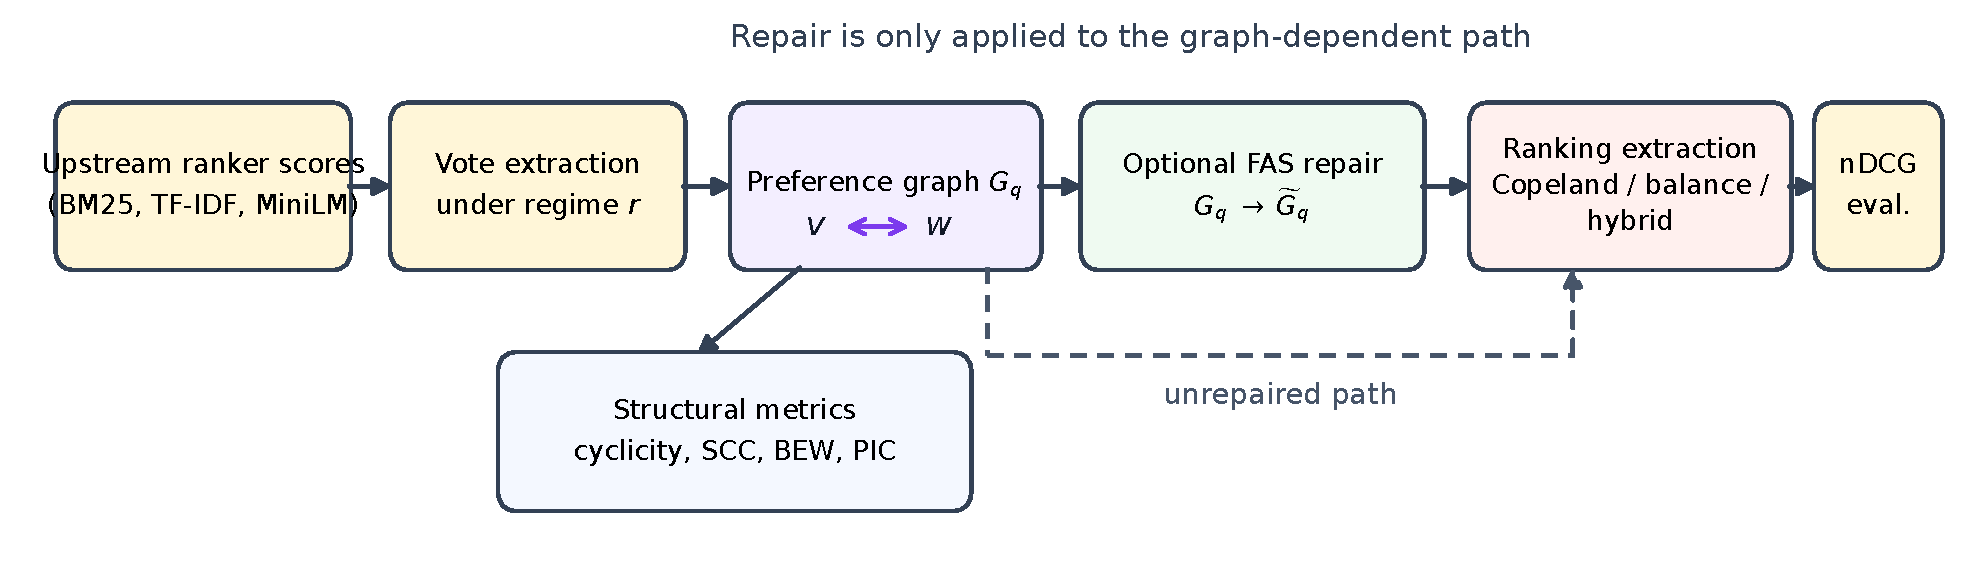
\includegraphics[width=0.98\linewidth]{../../../figures/manuscript/fig_pipeline.pdf}
  \caption{Preference-graph data-quality evaluation pipeline: upstream ranker
    scores $\to$ vote extraction under a regime $r$ $\to$ preference graph
    $G_q$ $\to$ structural metrics $\to$ optional FAS repair producing
    $\widetilde G_q$ $\to$ ranking extraction (Copeland / balance / hybrid) on
    either $G_q$ or $\widetilde G_q$ $\to$ nDCG evaluation.}
  \Description{Left-to-right pipeline diagram showing upstream ranker scores,
    vote extraction under a regime, a preference graph with a small directed
    cycle, optional feedback-arc-set repair on the graph-dependent path,
    structural metrics computed from the graph, ranking extraction, and final
    nDCG evaluation. A dashed unrepaired path bypasses the repair step.}
  \label{fig:pipeline}
\end{figure}

\subsection{Vote Extraction and Graph Construction}
\label{sec:vote-extraction}

Graph construction begins from per-ranker document scores, not from
pairwise judgments collected directly. For each query $q$ and each
constituent ranker $s$, and for every unordered candidate pair $\{u,v\}
\subset D_q$, ranker $s$ casts a directional \emph{vote} for whichever of
$u,v$ it scores higher, with vote weight equal to the ranker's own score
margin $|score_s(u) - score_s(v)|$; a ranker abstains from a pair if either
document is missing from its score list, or if its margin on that pair falls
below a fixed per-vote threshold. Votes are then aggregated per unordered
pair and per direction: for a candidate direction $(u,v)$, let
$\mathrm{support}(u,v)$ be the number of rankers voting for that direction and
$\mathrm{margin\_sum}(u,v)$ the sum of their margins. A directed edge
$(u,v)$ is retained in $E_q$, with weight $w_q(u,v)=\mathrm{margin\_sum}(u,v)$,
only if
\begin{equation}
  \mathrm{support}(u,v) \;\ge\; \tau_{\mathrm{sup}}
  \quad\text{and}\quad
  \mathrm{margin\_sum}(u,v) \;\ge\; \tau_{\mathrm{marg}},
  \label{eq:retention-rule}
\end{equation}
where the thresholds $\tau_{\mathrm{sup}}$ (minimum support) and
$\tau_{\mathrm{marg}}$ (minimum aggregate margin) are fixed per
vote-extraction regime $r$ (Section~\ref{sec:regimes}). Because both
directions of an unordered pair are evaluated independently under
Eq.~\eqref{eq:retention-rule}, a pair can retain edges in \emph{both}
directions when rankers disagree and each direction separately clears the
threshold; this is the mechanism by which cycles enter $G_q$. Candidate
documents are pooled across rankers by reciprocal rank
fusion~\cite{cormack2009rrf} before vote extraction, so $D_q$ is a shared set
regardless of which individual rankers surface which documents.

\subsection{Vote-Extraction Regimes}
\label{sec:regimes}

We construct three graphs per query from the same underlying ranker scores,
differing only in $(\tau_{\mathrm{sup}}, \tau_{\mathrm{marg}})$ and one
post-processing step, which we refer to as \emph{regimes}:

\begin{itemize}
  \item \textbf{\texttt{ms2}} (conservative): $\tau_{\mathrm{sup}}=2$,
    $\tau_{\mathrm{marg}}=0.1$. A direction is retained only with majority
    ranker support and a non-trivial aggregate margin, which suppresses most
    single-ranker disagreements.
  \item \textbf{\texttt{ms1}} (permissive): $\tau_{\mathrm{sup}}=1$,
    $\tau_{\mathrm{marg}}=0.0$. Every ranker-supported direction is retained,
    so both directions of a pair can coexist whenever rankers disagree.
  \item \textbf{\texttt{ms1\_drop\_mutual}}: built from the \texttt{ms1}
    output by deleting \emph{all} edges for any unordered pair that retained
    both directions, treating mutual disagreement as unresolved rather than
    keeping either arc.
\end{itemize}

These three regimes hold the upstream ranker scores fixed and vary only the
rule by which disagreement becomes graph structure, which lets us attribute
differences in graph cyclicity (Section~\ref{sec:structural-metrics}) to the
extraction rule rather than to the underlying evidence.

\subsection{Structural Data-Quality Metrics}
\label{sec:structural-metrics}

We measure four structural properties of a preference graph $G_q$: whether
it is acyclic (a binary indicator), the size of its largest strongly
connected component (a graph with no cycles has all components of size 1),
its edge count, and, for repair specifically, the total weight of edges a
repair operation removes (Section~\ref{sec:repair}). We additionally define
two metrics that relate a graph or ranking to an external reference ranking
$\pi_{\mathrm{ref}}$ (in our experiments, a ranking derived from relevance
judgments): the \textbf{backward-edge weight}
\begin{equation}
  \mathrm{BEW}(\pi_{\mathrm{ref}}, G) \;=\!\! \sum_{(u,v)\in E:\ \pi_{\mathrm{ref}}(v) < \pi_{\mathrm{ref}}(u)} \!\! w(u,v),
  \label{eq:bew}
\end{equation}
summing the weight of every edge $(u,v)$ (asserting $u\succ v$) that
$\pi_{\mathrm{ref}}$ contradicts by ranking $v$ ahead of $u$, and the
\textbf{pairwise inconsistency count}
\begin{equation}
  \mathrm{PIC}(\pi_{\mathrm{ref}}, G) \;=\; \bigl|\{(u,v)\in E : \pi_{\mathrm{ref}}(v) < \pi_{\mathrm{ref}}(u)\}\bigr|,
  \label{eq:pic}
\end{equation}
the unweighted count of the same contradictions. BEW and PIC are
graph-versus-reference diagnostics, not properties of a graph alone; when the
reference ranking is derived from the same relevance judgments used to
compute nDCG (Section~\ref{sec:retrieval-metrics}), this introduces a
circularity that we flag explicitly rather than treat as an independent
validation of structural repair (Section~\ref{sec:threats}, forward
reference).

\subsection{Graph Repair}
\label{sec:repair}

Repair is a single, well-defined operation on a graph: given $G_q$, find a
feedback arc set $F\subseteq E_q$ minimizing removed weight subject to
acyclicity of the remainder,
\begin{equation}
  F^\star \;=\; \operatorname*{arg\,min}_{F \subseteq E_q \,:\ (V_q,\, E_q\setminus F)\ \text{acyclic}} \ \sum_{(u,v)\in F} w_q(u,v),
  \label{eq:mwfas}
\end{equation}
and return $\widetilde G_q = (V_q, E_q\setminus F^\star, w_q)$. If $G_q$ is
already acyclic, $F^\star=\emptyset$ and $\widetilde G_q = G_q$. Solving
Eq.~\eqref{eq:mwfas} exactly is NP-hard in
general~\cite{ailon2008aggregating}; our main experiments use a greedy
heuristic with no approximation guarantee, not an exact solver: repeatedly
locate any directed cycle, remove its minimum-weight edge, and continue until
no cycle remains. This is a simple cycle-peeling procedure, not a claim of
optimality, and we compare it against stronger repair variants in
Section~\ref{sec:experimental-setup} to test whether the specific choice of
heuristic changes our conclusions. We report the total weight
$\sum_{(u,v)\in F^\star} w_q(u,v)$ removed by repair as a direct measure of
how much repair had to do on a given graph; when this quantity is zero,
repair is structurally inactive and $\widetilde G_q = G_q$ by construction.

Repair is defined purely in terms of $w_q$ and does not reference any
external relevance signal. This is the structural fact underlying the
Background section's argument (Section~\ref{sec:background}): nothing in
Eq.~\eqref{eq:mwfas} constrains whether the edges it removes are relevant,
irrelevant, or misleading with respect to a downstream retrieval metric.

\subsection{Ranking Extraction}
\label{sec:extraction}

Ranking extraction is a separate operation that consumes a graph (either
$G_q$ or $\widetilde G_q$) and produces a ranking $\pi$ of $V_q$; the same
extraction rule is applied regardless of which graph it receives, so repair
and extraction can be varied independently. We use two graph-derived
component scores. The \textbf{Copeland score} is out-degree minus in-degree,
\begin{equation}
  s_{\mathrm{cop}}(u) \;=\; \deg^+(u) - \deg^-(u),
  \label{eq:copeland}
\end{equation}
counting net wins irrespective of edge weight. The \textbf{weighted balance
score} is the signed sum of incident edge weight,
\begin{equation}
  s_{\mathrm{bal}}(u) \;=\; \sum_{(u,v)\in E} w(u,v) \;-\; \sum_{(v,u)\in E} w(v,u).
  \label{eq:balance}
\end{equation}
Both scores are well-defined on a graph with cycles---neither requires
acyclicity, since they are computed from local degree and weight sums rather
than from a topological order. This is what makes it possible to compute
$s_{\mathrm{cop}}$ and $s_{\mathrm{bal}}$ on the \emph{unrepaired} graph
$G_q$ directly, without first forcing an arbitrary tie-break on its cycles.

The primary ranking methods we evaluate are hybrids that combine one of
these two component scores with a query's prior ranking, obtained by
reciprocal rank fusion~\cite{cormack2009rrf} of the constituent rankers'
score lists. Writing $\hat{s}(\cdot)$ for min--max normalization of a score
vector to $[0,1]$ over the candidate set (so components on different native
scales are comparable), the hybrid score is
\begin{equation}
  s_{\mathrm{hybrid}}(u) \;=\; \hat{s}_{\mathrm{prior}}(u) \;+\; \alpha\, \hat{s}_{\mathrm{comp}}(u),
  \qquad \mathrm{comp} \in \{\mathrm{cop}, \mathrm{bal}\},
  \label{eq:hybrid}
\end{equation}
with $\alpha=0.3$ throughout the main experiments, and the extracted ranking
$\pi$ sorts $V_q$ by descending $s_{\mathrm{hybrid}}$, breaking exact ties
deterministically by document id. Applying Eq.~\eqref{eq:hybrid} with
$s_{\mathrm{comp}}$ computed on $G_q$ yields the \emph{unrepaired} hybrid
ranking for that component; applying it with $s_{\mathrm{comp}}$ computed on
$\widetilde G_q$ yields the \emph{repaired} hybrid ranking. The two rankings
differ only through $s_{\mathrm{comp}}$, since $\hat{s}_{\mathrm{prior}}$ and
$\alpha$ are identical in both cases---so any difference in downstream nDCG
between the repaired and unrepaired hybrid is attributable to repair changing
$s_{\mathrm{comp}}$, not to a change in how the ranking is extracted from a
score.

\subsection{Retrieval Metric}
\label{sec:retrieval-metrics}

Retrieval quality is measured by normalized discounted cumulative gain at
cutoff $k$. For a ranking $\pi$ and a relevance map $\mathrm{rel}:D_q\to
\mathbb{Z}_{\ge 0}$,
\begin{equation}
  \mathrm{nDCG@}k(\pi) \;=\; \frac{\displaystyle\sum_{i=1}^{k} \frac{2^{\mathrm{rel}(\pi_i)}-1}{\log_2(i+1)}}
  {\displaystyle\sum_{i=1}^{k} \frac{2^{\mathrm{rel}(\pi_i^{\mathrm{ideal}})}-1}{\log_2(i+1)}},
  \label{eq:ndcg}
\end{equation}
where $\pi_i$ is the document at rank $i$ in $\pi$ and $\pi^{\mathrm{ideal}}$
sorts all judged documents by descending relevance; nDCG@$k$ is defined as
$0$ when the ideal-ranking denominator is $0$ (no relevant documents judged
for the query). Eq.~\eqref{eq:ndcg} is the only retrieval-effectiveness
metric used for the main comparisons in this paper; it is entirely
independent of the graph-internal metrics of
Section~\ref{sec:structural-metrics}, which is the property that makes it
possible to ask, rather than assume, whether repair helps retrieval.

% =============================================================================
\section{Experimental Setup}
\label{sec:experimental-setup}
% Written from scratch and verified against scripts/run_publication_vote_suite.py,
% scripts/build_votes_file.py, scripts/run_real_experiment.py,
% experiments/final_method_gap_audit_20260711_221113/run_final_method_gap_audit.py,
% experiments/method_improvement_audit_20260711_205733/run_method_improvement_audit.py,
% and scripts/bootstrap_method_deltas.py during this pass.

\subsection{Datasets}
\label{sec:datasets}

We use four public retrieval benchmarks spanning distinct domains: SciDocs
(scientific document retrieval)~\cite{cohan2020scidocs}, FiQA (financial
opinion and question answering)~\cite{maia2018fiqa}, HotpotQA (multi-hop
question answering)~\cite{yang2018hotpotqa}, and BRIGHT (reasoning-intensive
retrieval)~\cite{su2024bright}. SciDocs, FiQA, and HotpotQA additionally
appear in the BEIR zero-shot retrieval benchmark
suite~\cite{thakur2021beir}; BRIGHT is a more recent addition designed
specifically to stress-test retrieval under reasoning-heavy queries. A query
is eligible for our protocol only if its relevance judgments support ranking
comparison: either multi-grade judgments over at least two documents with at
least two distinct grades, or at least one judged document with strictly
positive relevance (the shallower, positive-only judgment style common to
several BEIR-derived exports). Eligible queries without an eligible query
identifier list supplied externally are selected up to a per-dataset budget;
Table~\ref{tab:dataset-stats} reports the number of queries that yield a
non-empty vote-extraction result under each regime (Section~\ref{sec:regimes})
for each dataset. Counts differ slightly across regimes and datasets because
eligibility and vote extraction are both applied per query: a query can be
eligible for evaluation but still contribute no votes under a given
regime's thresholds if no candidate pair clears them.

\begin{table}[t]
  \caption{Number of queries per dataset and vote-extraction regime,
    from the four-dataset evaluation described in
    Section~\ref{sec:datasets}.}
  \label{tab:dataset-stats}
  \begin{tabular}{lccc}
    \toprule
    Dataset & \texttt{ms2} & \texttt{ms1} & \texttt{ms1\_drop\_mutual} \\
    \midrule
    SciDocs  & 119 & 120 & 120 \\
    FiQA     & 117 & 120 & 120 \\
    HotpotQA & 52  & 52  & 52  \\
    BRIGHT   & 34  & 50  & 50  \\
    \bottomrule
  \end{tabular}
\end{table}

\subsection{Rankers and Candidate Pooling}
\label{sec:rankers}

Upstream ranker scores come from three mechanical rankers: BM25, TF-IDF, and
a MiniLM cross-encoder. For each query, the candidate pool $D_q$ is formed by
reciprocal rank fusion~\cite{cormack2009rrf} of the three rankers' top-$n$
lists (retrieval depth $n\in\{35,50\}$ depending on dataset) down to a fixed
pool size $|D_q|\in\{10,20\}$ per dataset, and votes are then extracted over
$D_q$ as described in Section~\ref{sec:vote-extraction}, with a fixed
per-ranker abstention margin and abstention when a ranker lacks a score for
either candidate in a pair. We do not vary the ranker family across regimes
or datasets: \texttt{ms2}, \texttt{ms1}, and \texttt{ms1\_drop\_mutual} are
three views of the \emph{same} three rankers' scores, so any difference
between regimes reflects the vote-retention rule, not a change in evidence
source. We return to the scope this narrows the study to in
Section~\ref{sec:threats}: the main evidence base uses
mechanical, score-derived votes rather than direct human or LLM pairwise
judgments.

\subsection{Baselines}
\label{sec:baselines}

Table~\ref{tab:baselines} lists the ranking methods evaluated on the
four-dataset evaluation. The methods of primary interest are the four
repaired/unrepaired hybrid pairs (Section~\ref{sec:extraction},
Eq.~\eqref{eq:hybrid}), since these isolate the marginal effect of repair
while holding the prior ranking, the component score family, and $\alpha$
fixed. We additionally evaluate the prior ranking alone, and a set of
established fusion and graph-aggregation baselines that do not depend on
repair at all: reciprocal rank fusion~\cite{cormack2009rrf}, CombSUM~\cite{fox1994combination},
a Borda-count rank-aggregation baseline (points assigned by rank position,
summed across rankers), and a Rank-Centrality-style Markov chain
ranker~\cite{negahban2017rankcentrality} computed on the (unrepaired or
repaired) preference graph. CombSUM fuses per-ranker scores by summing, for
each candidate document, a per-(query, ranker) min--max normalization of
that ranker's score to $[0,1]$; a ranker that did not score a given document
contributes $0$ to that document's fused score, and exact ties are broken
first by the smallest rank the document achieved in any individual ranker's
own list, then by document id. The min--max normalization step is an
adaptation required by this study's heterogeneous ranker scales (BM25,
TF-IDF, a neural cross-encoder) and is not part of the original 1994
definition, which we note explicitly rather than presenting an adapted
baseline as an unmodified reproduction. These baselines answer a question
distinct from the repair-effect question: whether graph repair combined with
hybrid fusion is competitive with substantially simpler aggregation rules
that never inspect graph structure at all.

\begin{table}[t]
  \caption{Ranking methods evaluated in the four-dataset evaluation.
    ``Uses graph?'' indicates whether the method's score depends on the
    preference graph (as opposed to ranker scores alone); ``Repair
    variants?'' indicates whether the method is evaluated in both unrepaired
    and repaired form.}
  \label{tab:baselines}
  \begin{tabular}{lcc}
    \toprule
    Method & Uses graph? & Repair variants? \\
    \midrule
    Prior (RRF of BM25/TF-IDF/MiniLM) & No & --- \\
    Reciprocal rank fusion (RRF) & No & --- \\
    CombSUM & No & --- \\
    Borda-count fusion & No & --- \\
    Markov (Rank Centrality-style) & Yes & Yes \\
    Copeland hybrid (Eq.~\eqref{eq:hybrid}, comp.\ = Copeland) & Yes & Yes \\
    Balance hybrid (Eq.~\eqref{eq:hybrid}, comp.\ = balance) & Yes & Yes \\
    \bottomrule
  \end{tabular}
\end{table}

The three baselines marked ``No'' under ``Uses graph?'' in
Table~\ref{tab:baselines}---the prior ranking, reciprocal rank fusion, and
CombSUM (Borda-count fusion likewise)---depend only on the constituent
rankers' score files and are therefore invariant to vote-extraction regime:
their score for a given query is identical whether that query's graph is
built under \texttt{ms2}, \texttt{ms1}, or \texttt{ms1\_drop\_mutual}, since
regime only changes how the graph is constructed from those same scores.
When we report these baselines broken out by regime alongside the
graph-dependent methods, the repeated entries reflect the same underlying
score fused once and aligned across regimes for comparability, not
independent reruns or additional evidence; any aggregate statistic computed
over regime-labeled rows for a graph-independent baseline should be read
with this in mind.

A separate evaluation protocol (Section~\ref{sec:downstream-results})
assesses a wider pooled grid of twelve methods, including
the hybrids above, on a different query pool assembled for failure-taxonomy
analysis. We keep this pooled comparison clearly labeled as a distinct
protocol throughout the paper rather than merging its numbers with the
four-dataset evaluation above: the two protocols share method
implementations but not query sets, and reporting them as though they were
one evaluation would overstate the evidence either provides alone.

\subsection{Repair Variants Compared}
\label{sec:repair-variants}

Table~\ref{tab:repair-variants} lists the repair procedures we compare, both
fully reproducible from this repository alone. The \emph{greedy} heuristic
(Eq.~\eqref{eq:mwfas} solved by cycle-peeling, Section~\ref{sec:repair}) is
used throughout the main experiments. The second procedure applies an exact
solver---exhaustive enumeration of node orderings---to any strongly
connected component (SCC) with at most 10 nodes, and falls back to the same
greedy heuristic for larger components within the same query; we call this
combined procedure \emph{exact-for-small-components}, since it is exact only
on the (typically majority) share of SCCs at or below that size threshold and
is not a globally exact solver for the whole graph. Both procedures cover the
full four-dataset evaluation (all four datasets, all three regimes), not a
subsampled slice.

\begin{table}[t]
  \caption{Repair procedures compared (see text for reproducibility notes).}
  \label{tab:repair-variants}
  \begin{tabular}{p{4.3cm}p{2.9cm}}
    \toprule
    Procedure & Scope \\
    \midrule
    Greedy (cycle-peeling) & All queries; the repair method used throughout the main experiments \\
    Exact-for-small-components (brute-force, SCCs $\le 10$ nodes) + greedy fallback above that size & All queries \\
    \bottomrule
  \end{tabular}
\end{table}

This comparison is sufficient to test whether improving the graph-internal
structural objective (Eq.~\eqref{eq:mwfas}) more thoroughly than the greedy
heuristic translates into a retrieval-quality gain: exact-for-small-components
removes strictly at least as much backward edge weight as greedy on every
SCC it solves exactly, so if stronger optimization of the structural
objective were the limiting factor in Section~\ref{sec:downstream-results}'s null and mixed retrieval results, this comparison would
be expected to show it. We additionally ran a bounded robustness check
against several further exact and metaheuristic feedback-arc-set solvers on
a fixed sample of cyclic queries; it showed the same qualitative pattern
(stronger or exact repair did not translate into improved nDCG) with no
recorded failures. Because those additional solvers depend on a separate,
author-maintained software package withheld from citation during
double-blind review, we report this check qualitatively here rather than as
a further table row, and will provide the full citation, package identity,
and quantitative results in the camera-ready version and supplementary
material. Neither this repository's central conclusions nor
Section~\ref{sec:downstream-results}'s comparisons depend on that bounded
check: the two procedures in Table~\ref{tab:repair-variants} are the
evidentiary basis for every stronger-repair claim in this paper.

\subsection{Statistical Testing: Paired Bootstrap}
\label{sec:bootstrap}

Every repaired-versus-unrepaired comparison is evaluated with a paired,
per-query percentile bootstrap. For a method pair (e.g., repaired and
unrepaired Copeland hybrid) and a set of $n$ queries for which both methods
produced an nDCG@$k$ value, let $\delta_i = \mathrm{nDCG@}k_i^{\mathrm{repaired}}
- \mathrm{nDCG@}k_i^{\mathrm{unrepaired}}$ for query $i=1,\dots,n$. We draw
$B=2{,}000$ bootstrap resamples, each obtained by sampling $n$ query indices
independently and uniformly with replacement from $\{1,\dots,n\}$ and
averaging the corresponding $\delta_i$; writing $\bar\delta^{(b)}$ for the
mean of resample $b$, the reported interval is
\begin{equation}
  \left[\, \bar\delta^{(\lceil 0.025(B-1)\rceil)},\; \bar\delta^{(\lceil 0.975(B-1)\rceil)} \,\right],
  \label{eq:bootstrap-ci}
\end{equation}
the empirical 2.5th and 97.5th percentiles of the sorted resample means
$\bar\delta^{(1)}\le \cdots \le\bar\delta^{(B)}$, alongside the observed mean
$\bar\delta = \frac{1}{n}\sum_i \delta_i$. We use this percentile interval
throughout rather than a normal-approximation interval because many of the
per-query delta distributions are highly non-normal: in near-acyclic regimes
(Section~\ref{sec:regimes}), $\delta_i=0$ for every query, and the resample
distribution is a point mass at zero rather than anything a normal
approximation would describe well. All confidence intervals reported in this
paper use $B=2{,}000$ unless stated otherwise.

\subsection{Implementation, Hardware, and Resource Measurement}
\label{sec:implementation}

The full evaluation procedure (vote extraction, graph construction, greedy
repair, ranking extraction, nDCG evaluation, and bootstrap analysis) is
implemented in Python (3.11/3.12) using \texttt{networkx} for graph
operations, and is reproducible end to end from the released code
(Section~\ref{sec:data-availability}).
Wall-clock timing is measured per pipeline stage with
\texttt{time.perf\_counter()} around each stage in isolation; we report
per-stage means over queries rather than a single end-to-end number, since
the stages have very different and dataset-dependent costs (repair
dominates on large, cyclic graphs; ranking extraction and evaluation are
comparatively cheap at every scale we test). Memory is measured as the
maximum of the process's resident set size (RSS) sampled immediately before
and immediately after a stage; this is a coarse before/after snapshot, not
instrumented peak-memory tracking (e.g., \texttt{tracemalloc}), and should be
read as an approximate, directional indicator rather than a precise memory
profile. All runtime and memory measurements in this paper were collected on
a single, unbenchmarked local development machine rather than a controlled or
standardized hardware configuration; we report relative comparisons across
methods run on the same machine rather than absolute figures intended to
generalize to other hardware. This repository additionally contains a
complete, self-contained integer-programming formulation of
Eq.~\eqref{eq:mwfas} that requires a commercial mixed-integer solver license
to run; it was not used to produce any result reported in this paper. Both
procedures in Table~\ref{tab:repair-variants} require neither a commercial
solver license nor any dependency outside this repository.

\subsection{Real-LLM Evidence: Scope and Role}
\label{sec:real-llm-scope}

In addition to the mechanical three-ranker evaluation described above, we
evaluate a small, bounded sample of real large-language-model judgments
(pairwise, pointwise, and listwise) on subsets of SciDocs, HotpotQA, and
FiQA, using the same repaired-versus-unrepaired comparison structure. We
describe the primary paired OpenAI pilot in Section~\ref{sec:real-llm}, and
we keep it separate from a second, protocol-distinct multi-provider
failure-mining corpus with Cohere/Azure pairwise judgments on FiQA,
HotpotQA, and BRIGHT. We flag this scope here because it is easy to conflate
any real-LLM evidence with the main mechanical-vote evaluation if the
protocols are not kept separate. The real-LLM sample is one to two orders of
magnitude smaller than the main evaluation (tens of queries per dataset
rather than dozens to low hundreds), and is reported throughout this paper
as a bounded check on whether the regime-conditional pattern of
Sections~\ref{sec:structural-results}
and~\ref{sec:downstream-results} persists under a qualitatively different
preference source---not as independent confirmatory evidence at the same
scale or standard of certainty as the main evaluation.

% =============================================================================
\section{Structural Data Quality Results}
\label{sec:structural-results}

Table~\ref{tab:structural-results} reports the structural metrics defined in
Section~\ref{sec:structural-metrics} for all four datasets under all three
vote-extraction regimes.

\begin{table}[t]
  \caption{Structural metrics by dataset and vote-extraction regime. Cyclic\%
    is the share of query graphs containing at least one directed cycle;
    Largest SCC is the mean size of the largest strongly connected component.
    Source: \texttt{table\_graph\_ndcg\_and\_consistency.csv}.}
  \label{tab:structural-results}
  \begin{tabular}{llcc}
    \toprule
    Dataset & Regime & Cyclic\% & Largest SCC \\
    \midrule
    SciDocs  & \texttt{ms2}               & 0.0  & 1.00 \\
    SciDocs  & \texttt{ms1}               & 87.5 & 9.33 \\
    SciDocs  & \texttt{ms1\_drop\_mutual} & 0.0  & 1.00 \\
    FiQA     & \texttt{ms2}               & 0.0  & 1.00 \\
    FiQA     & \texttt{ms1}               & 95.0 & 12.51 \\
    FiQA     & \texttt{ms1\_drop\_mutual} & 0.0  & 1.00 \\
    HotpotQA & \texttt{ms2}               & 0.0  & 1.00 \\
    HotpotQA & \texttt{ms1}               & 51.9 & 2.52 \\
    HotpotQA & \texttt{ms1\_drop\_mutual} & 0.0  & 1.00 \\
    BRIGHT   & \texttt{ms2}               & 0.0  & 1.00 \\
    BRIGHT   & \texttt{ms1}               & 60.0 & 6.48 \\
    BRIGHT   & \texttt{ms1\_drop\_mutual} & 6.0  & 1.40 \\
    \bottomrule
  \end{tabular}
\end{table}

The regime contrast is stark and uniform across datasets. Under \texttt{ms2},
every dataset is effectively acyclic (0\% cyclic queries, largest SCC $=1.0$);
under \texttt{ms1}, cyclic-query prevalence rises to 51.9--95.0\% with largest
SCC 2.5--12.5, an order-of-magnitude structural change from the same
underlying ranker scores. \texttt{ms1\_drop\_mutual} restores near-acyclicity
on three of four datasets; BRIGHT retains a small residual (6.0\% cyclic,
largest SCC $1.4$), the one partial exception to an otherwise clean pattern.
Figure~\ref{fig:cyclicity-scc} shows this contrast graphically. Because the
three regimes share identical upstream ranker scores (Section~\ref{sec:regimes}),
this difference is attributable to the vote-retention rule alone, not to any
change in evidence quality --- the central structural finding of this study is
that \emph{construction}, not repair, is the dominant lever on preference-graph
consistency.

\begin{figure}[t]
  \centering
  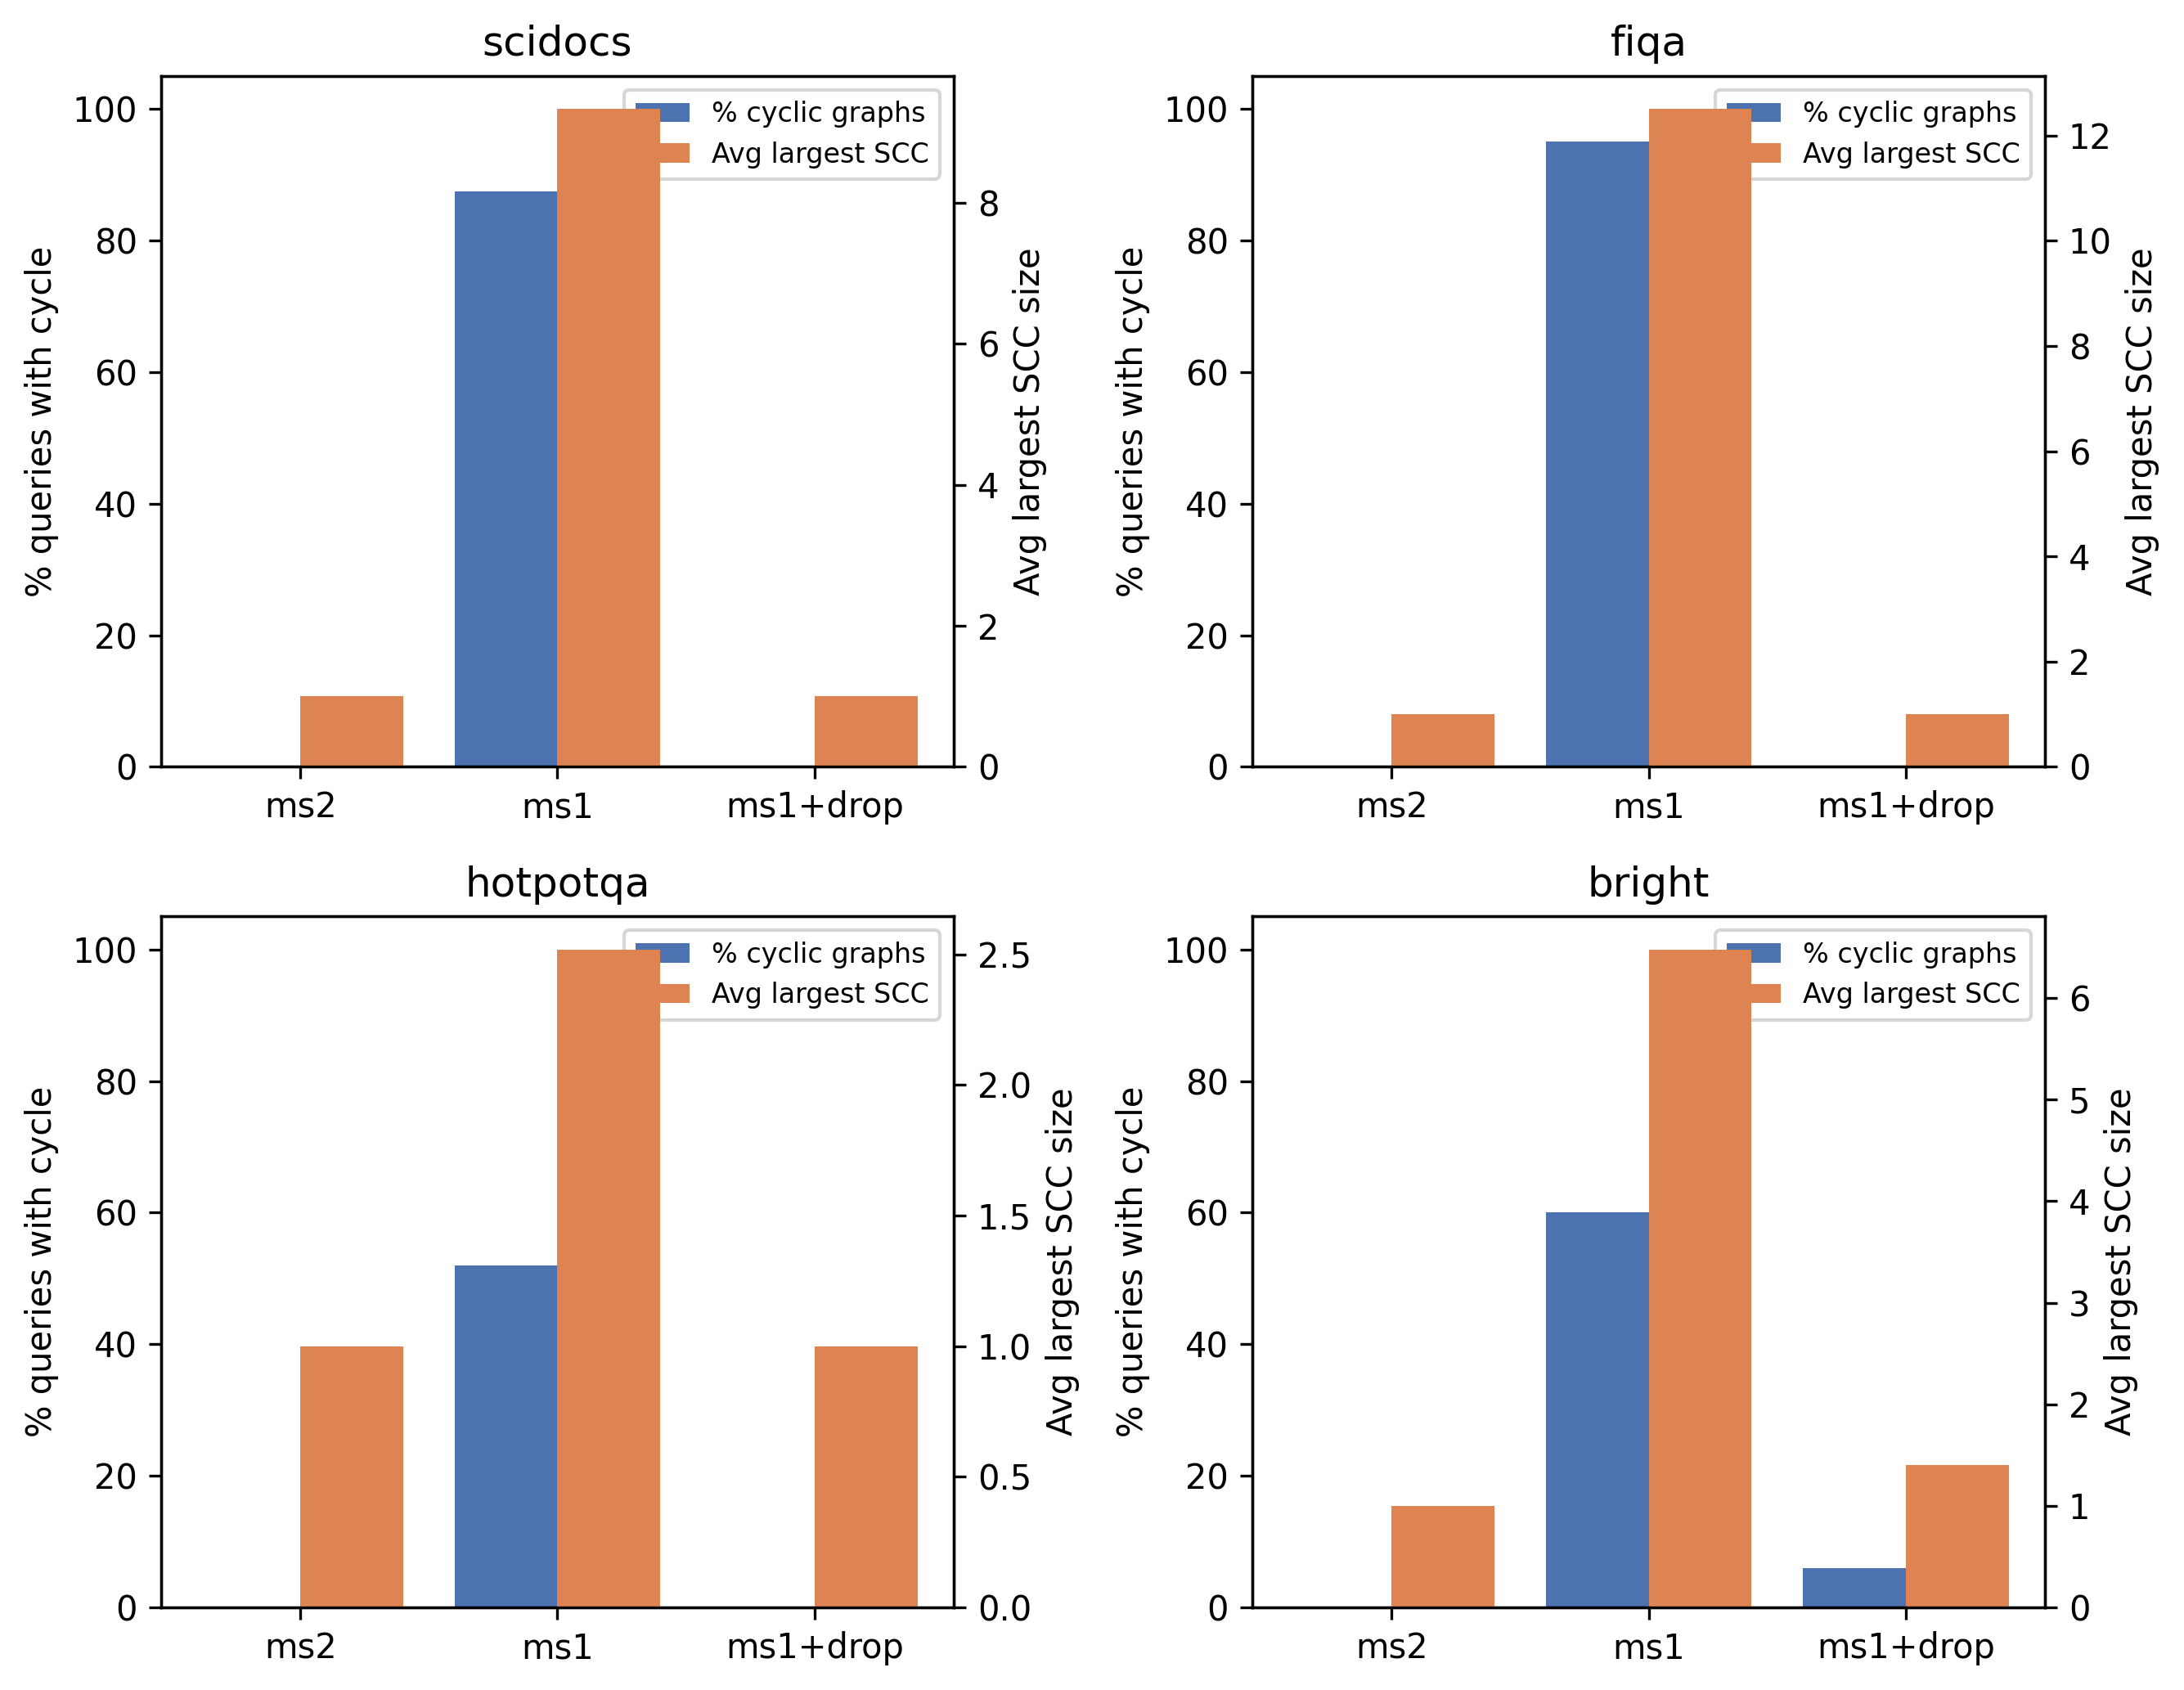
\includegraphics[width=0.95\linewidth]{../../../figures/manuscript/fig_cyclicity_and_scc.png}
  \caption{Percentage of cyclic query graphs and mean largest strongly
    connected component size, by dataset and vote-extraction regime.
    \texttt{ms2} and \texttt{ms1\_drop\_mutual} are near-acyclic on every
    dataset; \texttt{ms1} is substantially cyclic on all four, with HotpotQA
    showing the mildest effect and FiQA the strongest.}
  \Description{Grid of four panels, one per dataset (SciDocs, FiQA, HotpotQA,
    BRIGHT). Each panel shows three vote-extraction regimes (ms2, ms1, ms1
    drop mutual) on the horizontal axis, with two bars per regime on a
    dual y-axis: percentage of cyclic query graphs (left axis) and mean
    largest strongly connected component size (right axis). In every panel,
    ms1 bars are substantially higher on both axes than ms2 and ms1 drop
    mutual, which are at or near zero; FiQA shows the highest ms1 cyclicity
    (about 95 percent) and HotpotQA the lowest (about 52 percent).}
  \label{fig:cyclicity-scc}
\end{figure}

Repair acts only where cyclicity is present, so its structural effect is
concentrated in \texttt{ms1}. Table~\ref{tab:bew-pic} reports mean
backward-edge weight (BEW, Eq.~\eqref{eq:bew}) and pairwise inconsistency
count (PIC, Eq.~\eqref{eq:pic}) before and after repair, computed against a
ranking derived from relevance judgments, together with the mean FAS weight
removed (Section~\ref{sec:repair}).

\begin{table}[t]
  \caption{Mean BEW and PIC before and after FAS repair, and mean FAS weight
    removed, under \texttt{ms1} (the only regime with material cyclicity;
    \texttt{ms2}/\texttt{ms1\_drop\_mutual} remove $\approx 0$ weight by
    construction). Source: \texttt{table\_consistency\_qrels\_bew.csv}.}
  \label{tab:bew-pic}
  \begin{tabular}{lccc}
    \toprule
    Dataset & $\Delta$BEW & $\Delta$PIC & Weight removed \\
    \midrule
    SciDocs  & 0.333 & 4.25 & 0.682 \\
    FiQA     & 0.472 & 6.22 & 1.099 \\
    HotpotQA & 0.035 & 0.50 & 0.121 \\
    BRIGHT   & 0.234 & 2.76 & 0.388 \\
    \bottomrule
  \end{tabular}
\end{table}

Repair reduces PIC on all four datasets (0.5--6.2 fewer inconsistent pairs)
with corresponding non-zero FAS weight removed; BEW reductions are smaller in
absolute magnitude but consistently positive. Figure~\ref{fig:bew-pic} shows
the BEW pre/post pair graphically (PIC values are in Table~\ref{tab:bew-pic}
only). We emphasize a caveat that is essential to
how this result should be read: BEW and PIC are computed against a reference
ranking derived from the same relevance judgments later used to compute
nDCG@$k$ (Section~\ref{sec:retrieval-metrics}). Whenever we describe repair as
improving structural consistency, that improvement is being scored against the
same evaluation signal used downstream --- a genuine but qrels-anchored
diagnostic, not an independent measure of ground truth, and not by itself
evidence that a retrieval-quality gain must follow. Sections~\ref{sec:downstream-results}
and~\ref{sec:failure-taxonomy} test that separate question directly and find
that it does not follow uniformly.

\begin{figure}[t]
  \centering
  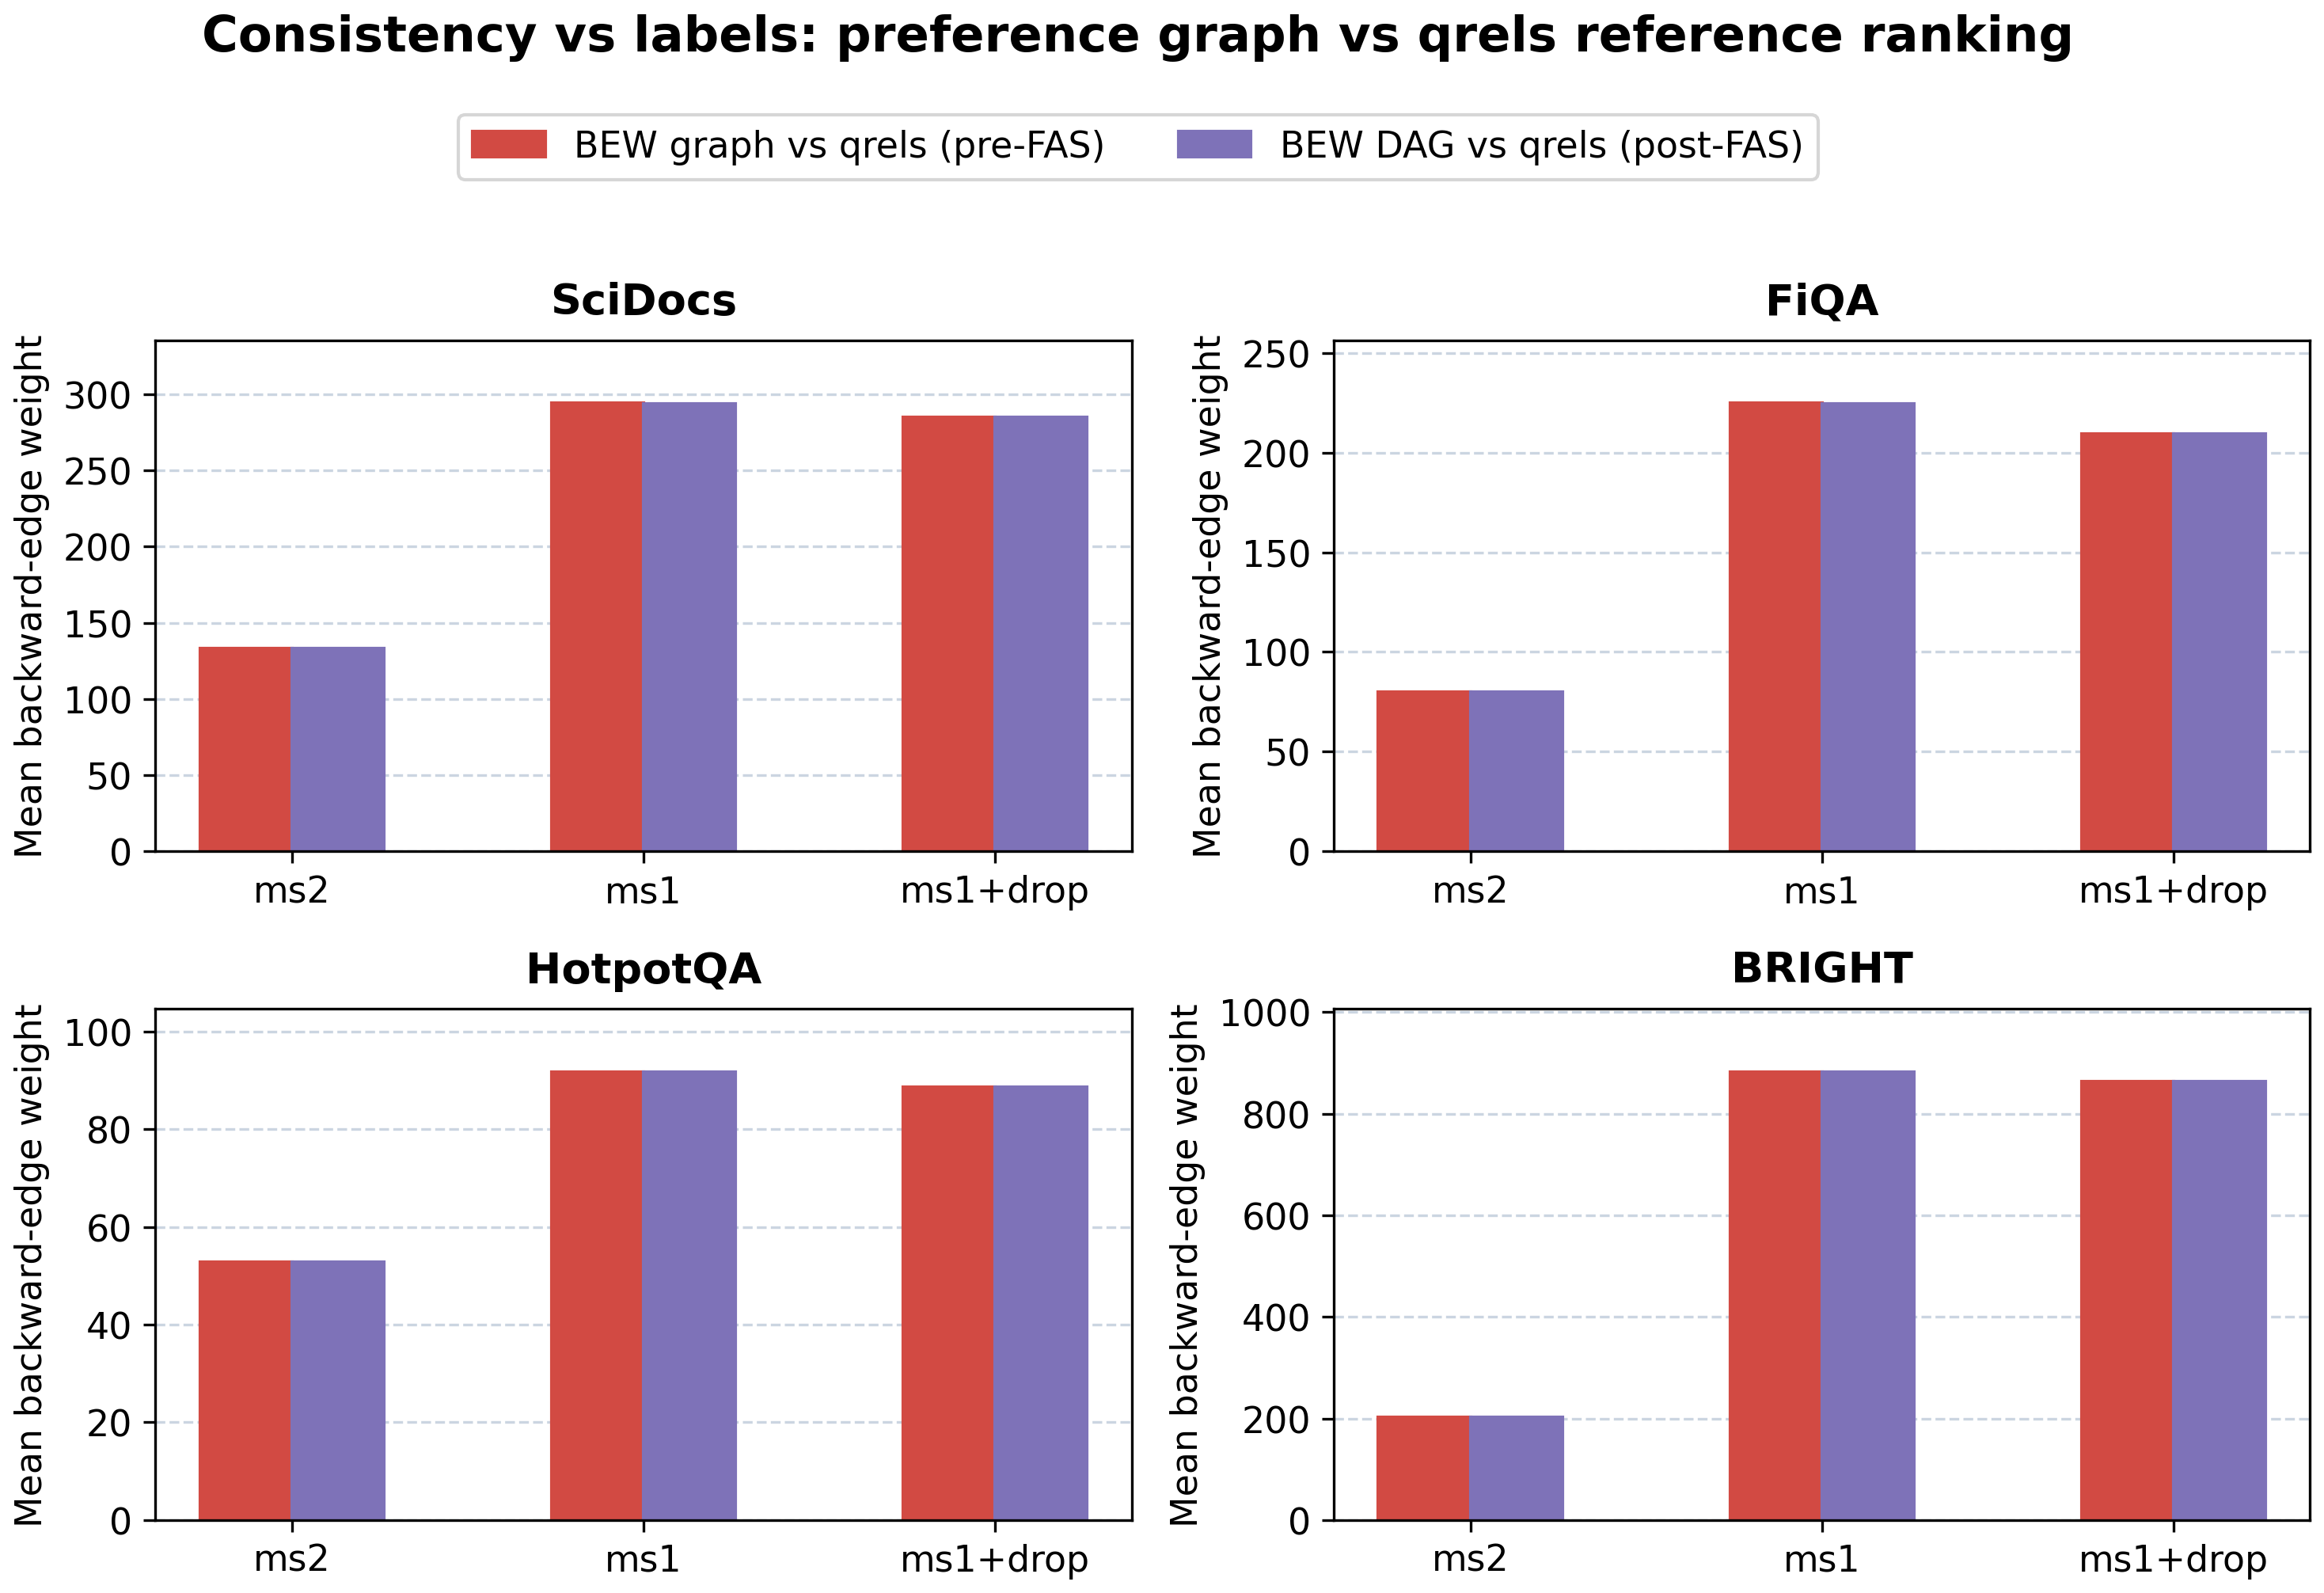
\includegraphics[width=0.95\linewidth]{../../../figures/manuscript/fig_graph_qrels_bew_pre_post.png}
  \caption{Mean backward-edge weight (BEW) before and after FAS repair, under
    \texttt{ms1}, for all four datasets (corresponding PIC values are reported
    in Table~\ref{tab:bew-pic} rather than plotted here). BEW is computed
    against the same relevance judgments used for downstream nDCG evaluation
    (Section~\ref{sec:retrieval-metrics}) and should be read as a structural
    diagnostic rather than an independent validation of repair quality.}
  \Description{Grid of four panels, one per dataset (SciDocs, FiQA, HotpotQA,
    BRIGHT). Each panel shows mean backward-edge weight against a qrels-derived
    reference ranking, before FAS repair and after FAS repair, for three
    vote-extraction regimes (ms2, ms1, ms1 drop mutual). Pre- and post-repair
    bars are nearly identical in height in every panel, reflecting the small
    magnitude of the backward-edge-weight reduction reported in
    Table~\ref{tab:bew-pic}.}
  \label{fig:bew-pic}
\end{figure}

% =============================================================================
\section{Downstream Quality Results: Repair vs.\ Retrieval}
\label{sec:downstream-results}

Section~\ref{sec:structural-results} established that repair measurably
improves structural consistency when the graph is cyclic. This section asks
the separate question motivating this study: does that structural
improvement translate into a retrieval-quality gain, measured by nDCG@$k$
(Eq.~\eqref{eq:ndcg})? We report the paired bootstrap comparison
(Section~\ref{sec:bootstrap}) for the repaired-versus-unrepaired Copeland and
balance hybrids (Eq.~\eqref{eq:hybrid}), then the pooled comparison against
fixed aggregation baselines, then the stronger-repair comparison already
introduced in Table~\ref{tab:repair-variants}.

\subsection{Repaired vs.\ Unrepaired Hybrids}

Table~\ref{tab:bootstrap-delta-ndcg} reports the bootstrap mean
$\Delta\mathrm{nDCG@}k$ (repaired minus unrepaired) for the Copeland hybrid
under all four datasets and three regimes; the corresponding balance-hybrid
row is degenerate at exactly $[0,0]$ in every one of the twelve cells and is
summarized rather than tabulated in full. Figure~\ref{fig:bootstrap-delta-ndcg}
plots all twenty-four cells (Copeland and balance) together.

\begin{table}[t]
  \caption{Bootstrap mean $\Delta$nDCG@$k$ (repaired $-$ unrepaired Copeland
    hybrid), with 95\% CI (2,000 resamples, Eq.~\eqref{eq:bootstrap-ci}).
    Source: \texttt{table\_bootstrap\_delta\_ndcg.csv}.}
  \label{tab:bootstrap-delta-ndcg}
  \begin{tabular}{llccc}
    \toprule
    Dataset & Regime & $n$ & Mean $\Delta$ & 95\% CI \\
    \midrule
    SciDocs  & \texttt{ms2}               & 119 & 0.0 & $[0, 0]$ \\
    SciDocs  & \texttt{ms1}               & 120 & $-0.0001$ & $[-0.0008, 0.0006]$ \\
    SciDocs  & \texttt{ms1\_drop\_mutual} & 120 & 0.0 & $[0, 0]$ \\
    FiQA     & \texttt{ms2}               & 117 & 0.0 & $[0, 0]$ \\
    FiQA     & \texttt{ms1}               & 120 & $+0.0015$ & $[-0.0005, 0.0042]$ \\
    FiQA     & \texttt{ms1\_drop\_mutual} & 120 & 0.0 & $[0, 0]$ \\
    HotpotQA & \texttt{ms2}               & 52  & 0.0 & $[0, 0]$ \\
    HotpotQA & \texttt{ms1}               & 52  & $\mathbf{+0.0167}$ & $\mathbf{[0, 0.0405]}$ \\
    HotpotQA & \texttt{ms1\_drop\_mutual} & 52  & 0.0 & $[0, 0]$ \\
    BRIGHT   & \texttt{ms2}               & 34  & 0.0 & $[0, 0]$ \\
    BRIGHT   & \texttt{ms1}               & 50  & $+0.00002$ & $[-0.0018, 0.0016]$ \\
    BRIGHT   & \texttt{ms1\_drop\_mutual} & 50  & 0.0 & $[0, 0]$ \\
    \bottomrule
  \end{tabular}
\end{table}

Twenty of the twenty-four dataset$\times$regime$\times$pair cells (Copeland
and balance combined) show an interval of exactly $[0,0]$: every \texttt{ms2}
and \texttt{ms1\_drop\_mutual} cell, and every balance-hybrid cell regardless
of regime. This is the direct retrieval-level consequence of
Section~\ref{sec:structural-results}'s structural finding --- when the graph
is already near-acyclic, repair removes negligible edge weight
(Table~\ref{tab:bew-pic}), and an intervention with nothing to act on cannot
change the ranking it produces. Among the four \texttt{ms1}/Copeland cells,
where the graph is substantially cyclic, three intervals straddle zero
(SciDocs, FiQA, BRIGHT); one, HotpotQA, has an interval bounded away from
negative (mean $+0.0167$, CI $[0, 0.0405]$) --- the only cell in the full
table where repair shows a retrieval effect distinguishable from noise. We
describe this interval as bounded away from negative rather than as
excluding zero, since its lower bound is exactly $0.0$: the appropriate
reading is that repair reliably does not hurt on HotpotQA \texttt{ms1} and
plausibly helps, not that a strictly positive effect has been established
with certainty. Notably, HotpotQA has the \emph{lowest} \texttt{ms1} cyclicity
(51.9\%) of the four datasets (Table~\ref{tab:structural-results}) --- the one
reliable retrieval effect does not come from the most structurally
inconsistent dataset, which weighs against a simple ``more cyclicity implies
more benefit from repair'' reading of these results.

\begin{figure}[t]
  \centering
  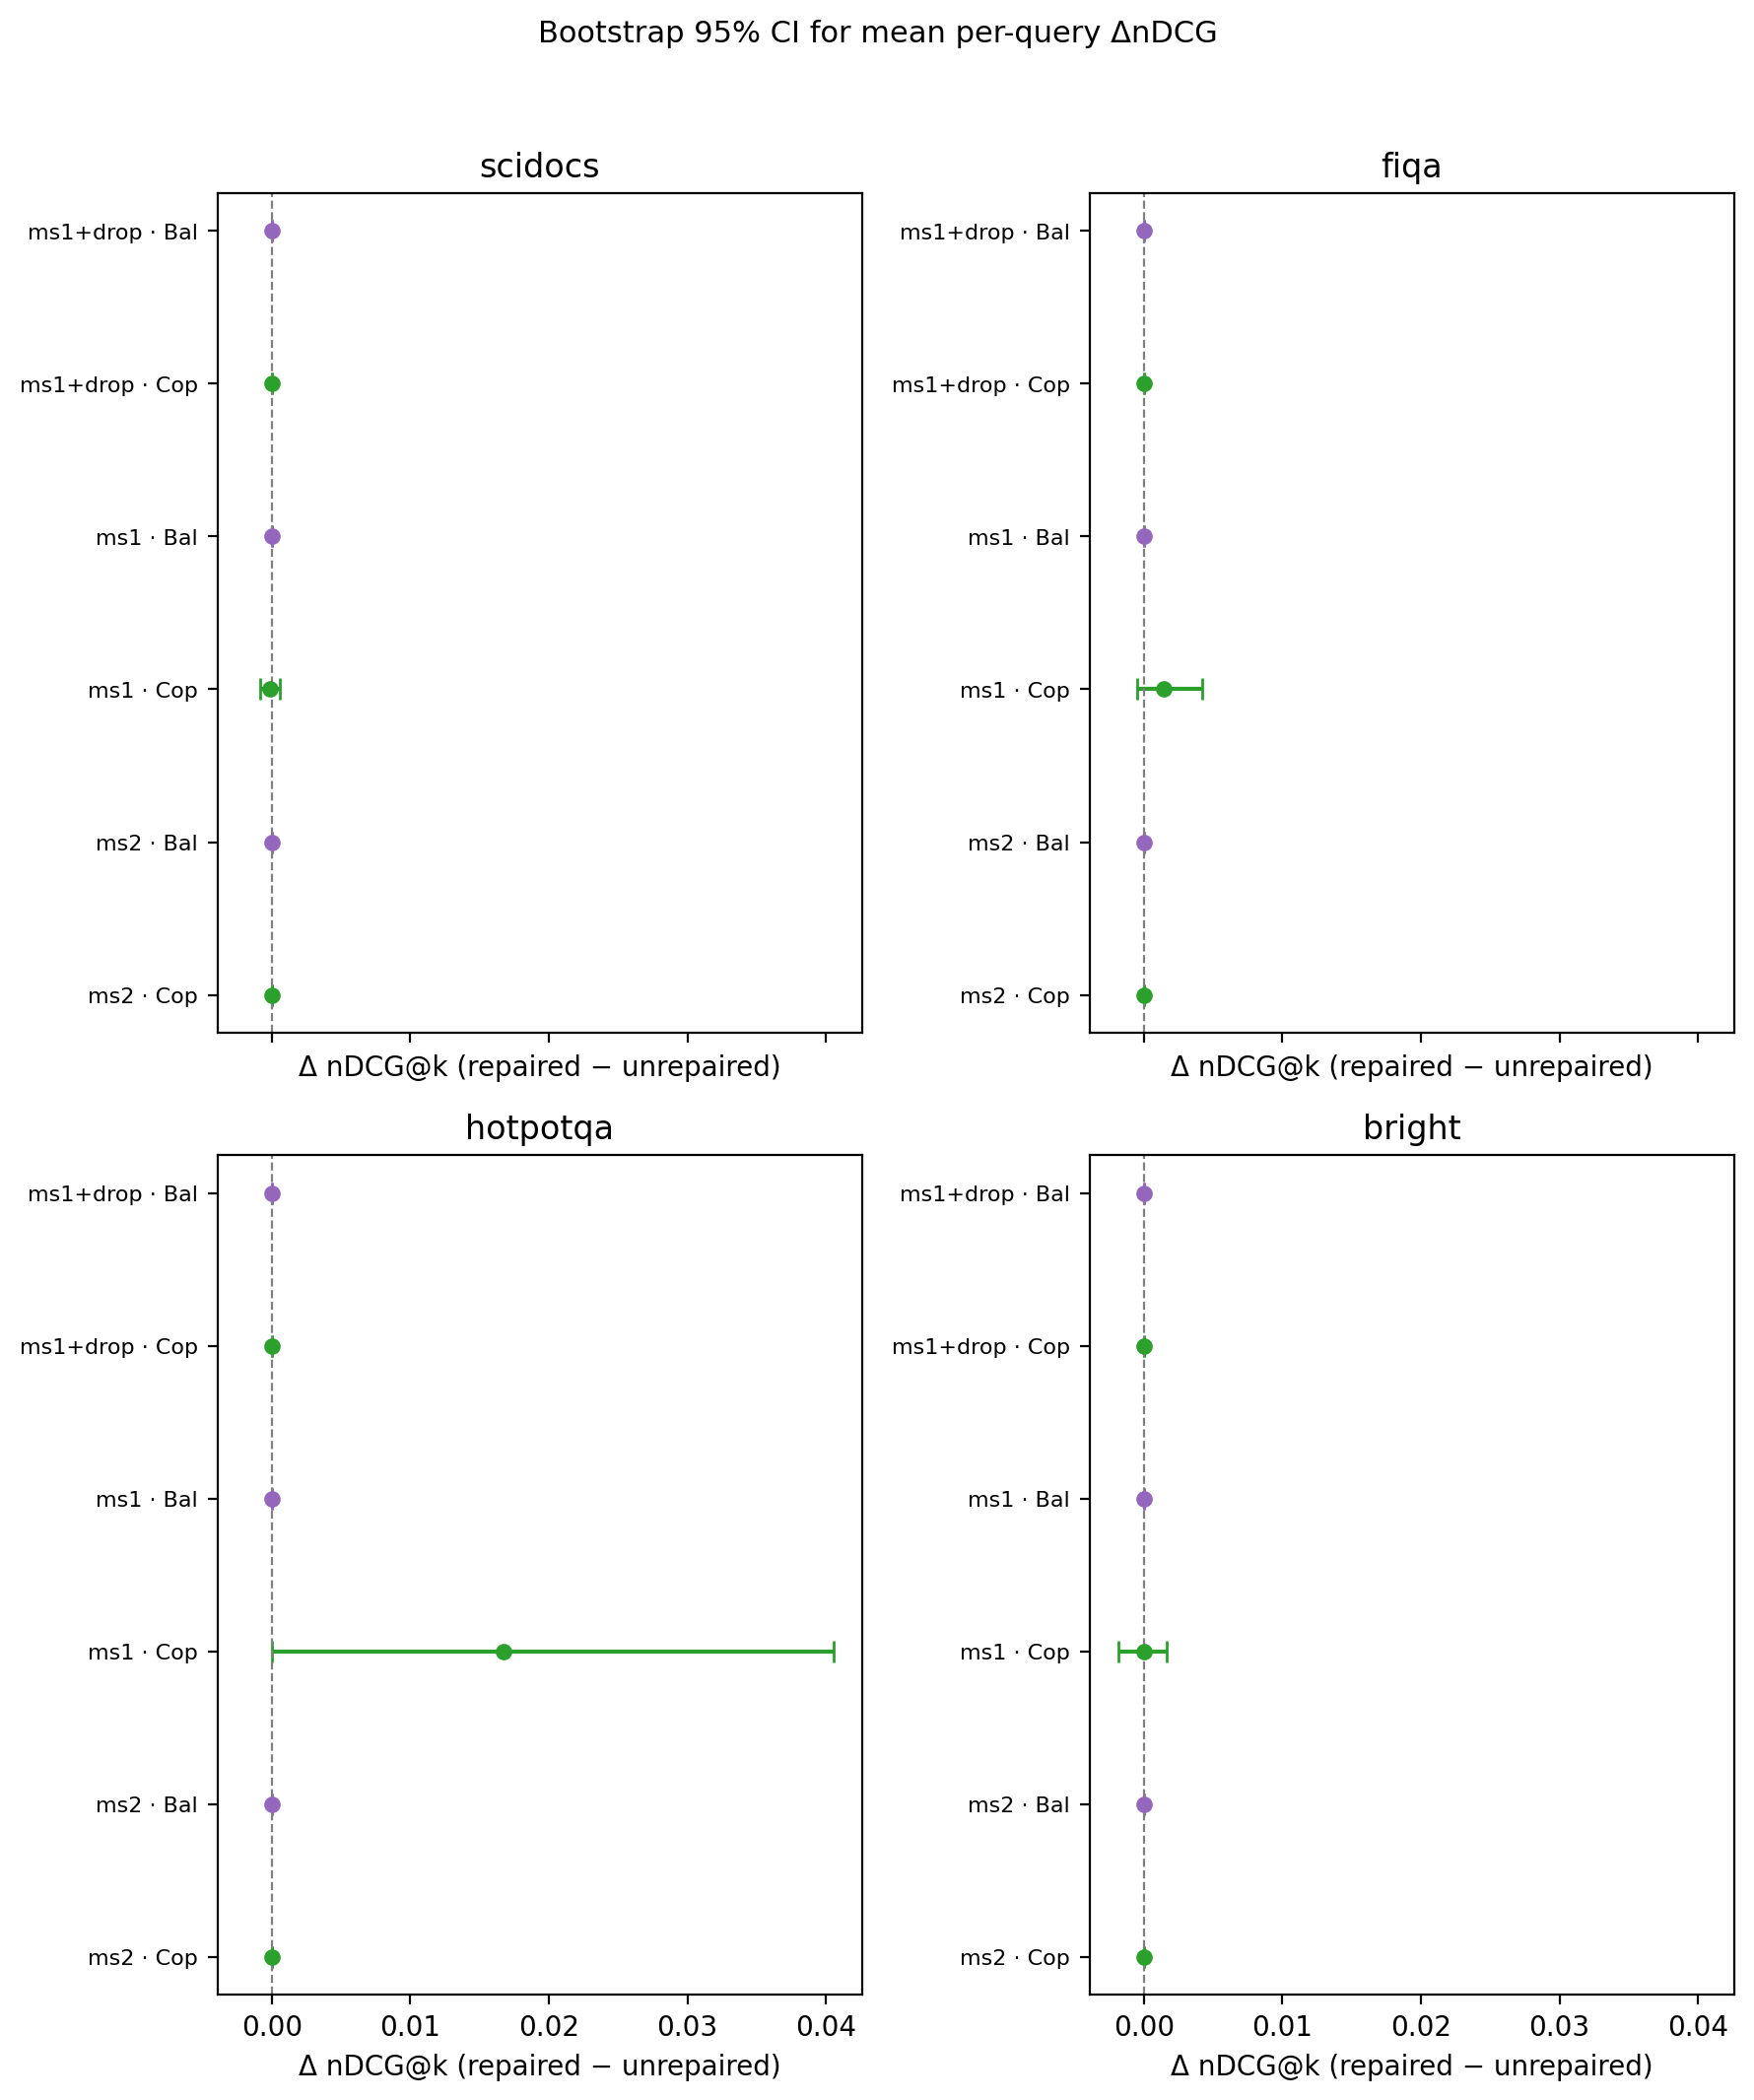
\includegraphics[width=0.95\linewidth]{../../../figures/manuscript/fig_delta_ndcg_bootstrap.png}
  \caption{Bootstrap mean $\Delta$nDCG@$k$ (repaired $-$ unrepaired hybrid
    ranking) with 95\% confidence intervals, for Copeland and balance hybrids,
    across four datasets and three vote-extraction regimes (24 cells total,
    six per dataset panel). Twenty cells are degenerate at $[0,0]$; among the
    four active \texttt{ms1}/Copeland cells, only HotpotQA's interval is
    bounded away from negative.}
  \Description{Grid of four forest-plot panels, one per dataset (SciDocs,
    FiQA, HotpotQA, BRIGHT). Each panel has six rows, one per combination of
    the three vote-extraction regimes (ms2, ms1, ms1 drop mutual) and the two
    hybrid pairs (Copeland, balance), showing the bootstrap mean difference in
    nDCG between repaired and unrepaired rankings with horizontal 95 percent
    confidence interval whiskers and a vertical dashed reference line at zero.
    In every panel, five of the six rows are points exactly at zero with
    zero-width intervals; the sixth row (ms1, Copeland) is non-degenerate in
    all four panels, and only in the HotpotQA panel does that row's interval
    not extend below zero.}
  \label{fig:bootstrap-delta-ndcg}
\end{figure}

\subsection{Comparison with Fixed Aggregation Baselines}

The comparison above isolates the marginal effect of repair while holding
fusion and extraction fixed. A separate question is whether the resulting
hybrid pipeline is competitive with simple aggregation rules that never
inspect graph structure at all. Table~\ref{tab:pooled-baseline} reports mean
nDCG@$k$ pooled over the 1,020-record failure-mining corpus
(Section~\ref{sec:baselines}) for twelve methods, and
Figure~\ref{fig:mean-ndcg-hybrids} visualizes the same pooled ordering with
marginal bootstrap intervals.

\begin{figure}[t]
  \centering
  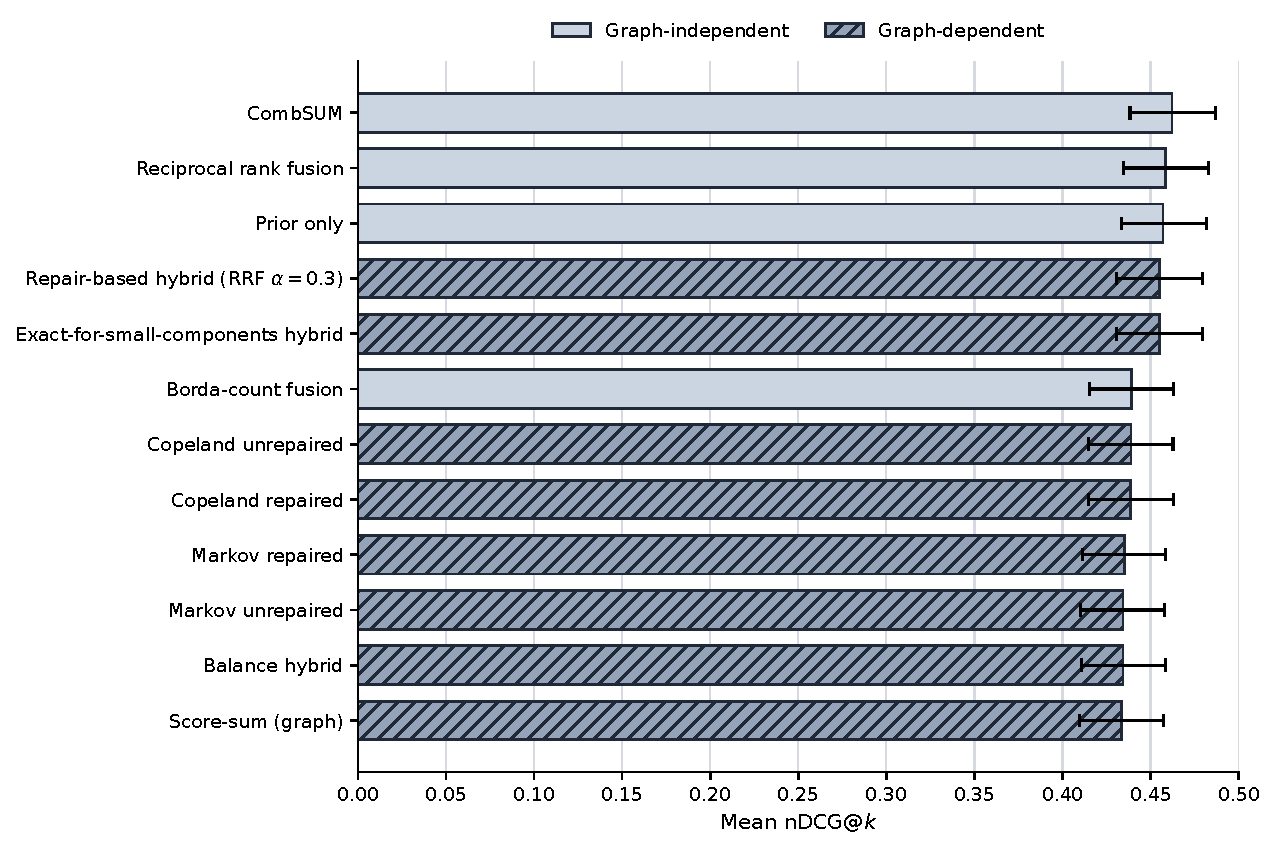
\includegraphics[width=0.98\linewidth]{../../../figures/manuscript/fig_mean_ndcg_hybrids.pdf}
  \caption{Pooled mean nDCG@$k$ by ranking method across 1,020
    query$\times$regime records from the failure-mining evaluation corpus.
    Error bars show 95\% bootstrap confidence intervals for each method's
    pooled mean. Methods are ordered by point estimate and grouped by whether
    their score depends on the preference graph. CombSUM and reciprocal rank
    fusion have the two highest pooled mean nDCG point estimates, followed by
    the prior ranking; all graph-dependent methods are lower by point
    estimate. The intervals shown are marginal method-wise confidence
    intervals, not paired tests between methods.}
  \Description{Horizontal bar chart of pooled mean nDCG at cutoff k for
    twelve ranking methods across 1,020 query-times-regime records. Methods
    are ordered from highest to lowest point estimate and grouped into
    graph-independent and graph-dependent families. Each bar has a 95 percent
    bootstrap confidence interval whisker. CombSUM is highest by point
    estimate, followed by reciprocal rank fusion and the prior ranking.}
  \label{fig:mean-ndcg-hybrids}
\end{figure}

\begin{table}[t]
  \caption{Pooled mean nDCG@$k$ by method, 1,020 query$\times$regime records
    (failure-mining protocol; Section~\ref{sec:baselines}). Source:
    \texttt{final\_baseline\_comparison.csv} (scope=pooled).}
  \label{tab:pooled-baseline}
  \begin{tabular}{lc}
    \toprule
    Method & Mean nDCG \\
    \midrule
    CombSUM                  & \textbf{0.462} \\
    Reciprocal rank fusion   & 0.459 \\
    Prior only               & 0.457 \\
    Proposed$^{\ast}$ hybrid (repaired balance/Copeland mix) & 0.455 \\
    Best stronger repair (Table~\ref{tab:repair-variants}) & 0.455 \\
    Borda-count fusion       & 0.439 \\
    Copeland, unrepaired     & 0.439 \\
    Copeland, repaired       & 0.439 \\
    Markov, repaired         & 0.435 \\
    Markov, unrepaired       & 0.434 \\
    Balance hybrid           & 0.434 \\
    Score-sum (graph)        & 0.433 \\
    \bottomrule
  \end{tabular}
\end{table}

\noindent$^{\ast}$We use ``proposed hybrid'' only as the pooled-comparison
method label inherited from the underlying data files, referring to the same
repair-based hybrid construction of Eq.~\eqref{eq:hybrid}; we do not
characterize this construction as a novel contribution of this paper (see
Section~\ref{sec:introduction}).

CombSUM and reciprocal rank fusion --- both graph-independent
(Section~\ref{sec:baselines}) --- achieve the highest and second-highest
pooled mean nDCG, ahead of every graph-based method including the repaired
Copeland hybrid and the repair-based hybrid construction evaluated in this
paper. The prior ranking alone also exceeds repaired Copeland. This is a
direct answer to whether graph repair combined with hybrid fusion is a
better retrieval strategy than substantially simpler alternatives: on this
pooled comparison, it is not. As noted in Section~\ref{sec:baselines},
CombSUM, RRF, Borda-count, and the prior ranking are regime-invariant by
construction, so their pooled $n$ reflects corpus completeness across
regime-labeled rows for the same underlying queries rather than independent
per-regime observations; this affects the precision of their own reported
estimates, not the validity of the ordering above, since every method in
Table~\ref{tab:pooled-baseline} is scored under the same protocol.

\subsection{Stronger Repair Does Not Change the Conclusion}

Table~\ref{tab:repair-variants} (Section~\ref{sec:repair-variants}) compares
the greedy heuristic against the exact-for-small-components procedure on the
full 1,020-record dataset. Exact-for-small-components removes
marginally less mean structural weight than greedy on this corpus (0.546 vs.\
0.547) --- the two are close enough that neither dominates the other in
practice on these graphs --- and the paired pooled Copeland nDCG difference
is effectively zero (mean $\Delta = -0.0000358$, 95\% CI $[-0.000107, 0.0]$).
Exact-for-small-components is exact only on strongly
connected components of at most 10 nodes, falling back to greedy above that
size; it is not a globally exact solver for the whole graph, and we do not
describe it as one. This comparison is, by itself, sufficient to answer
whether a stronger structural solver changes the paper's retrieval
conclusion: it does not. A further bounded robustness check against
additional exact and metaheuristic solvers, on a fixed sample of cyclic
queries, showed the same qualitative pattern with no recorded failures; those
additional solvers depend on a separate, author-maintained software package
withheld from citation during double-blind review, so we report this check
qualitatively rather than as a further table row, and will provide full
citation and quantitative detail in the camera-ready version.

% =============================================================================
\section{Failure Taxonomy and Diagnostic Analysis}
\label{sec:failure-taxonomy}

Section~\ref{sec:downstream-results} showed that repair's retrieval effect is
usually null and occasionally negative. This section asks why, decomposing
the same 1,020-record pooled corpus into six manually verified, mutually
exclusive failure classes (Table~\ref{tab:failure-taxonomy};
Figure~\ref{fig:failure-classes}).

\begin{table}[t]
  \caption{Manual failure-class taxonomy, 1,020 query$\times$regime records.
    Source: \texttt{manual\_failure\_summary.csv}.}
  \label{tab:failure-taxonomy}
  \begin{tabular}{lccc}
    \toprule
    Class & Count & \% & Mean $\Delta$nDCG \\
    \midrule
    Repair-inactive              & 652 & 63.9 & 0.000 \\
    Tail-only change             & 210 & 20.6 & 0.000 \\
    Wrong-direction repair       & 55  & 5.4  & $-0.034$ \\
    Metric-neutral change        & 54  & 5.3  & 0.000 \\
    Extraction-insensitivity     & 26  & 2.5  & $+0.014$ \\
    Unknown / mixed              & 23  & 2.3  & $+0.036$ \\
    \bottomrule
  \end{tabular}
\end{table}

\textbf{Repair-inactive} (63.9\%, the dominant class) covers cases where FAS
repair removes negligible or zero edge weight, so the repaired and unrepaired
rankings coincide by construction --- the direct query-level manifestation of
the near-acyclic regimes in Section~\ref{sec:structural-results}.
\textbf{Tail-only change} (20.6\%) covers cases where repair does alter the
underlying graph ranking, but only below the evaluation cutoff, leaving
nDCG@$k$ unchanged: the structural intervention is real but invisible to the
retrieval metric at the depth we score. \textbf{Metric-neutral change} (5.3\%)
covers cases where repair changes which documents occupy the top ranks
without changing their relevance grades, so nDCG is unaffected even though
the ranking itself differs. \textbf{Extraction-insensitivity} (2.5\%) covers
cases where the Copeland or balance scoring rule (Section~\ref{sec:extraction})
is itself insensitive to the specific edges repair removes, so the score
computed from the repaired graph reproduces the unrepaired ranking. Together,
these four classes --- 91.7\% of all records --- describe mechanisms by which
a structural intervention fails to reach the retrieval metric at all, not
mechanisms by which repair actively harms retrieval.

\textbf{Wrong-direction repair} (5.4\%) is the only class with a materially
negative mean $\Delta$nDCG ($-0.034$): here repair changes the ranking and the
change moves relevant documents down, not up. This is the class in which
repair is actively harmful, and it is a minority of cases even within the
already-small set of records where repair is retrieval-active at all.
\textbf{Unknown/mixed} (2.3\%) covers records that did not cleanly fit the
other five categories under manual review. The counterfactual analysis
underlying this taxonomy additionally finds that \emph{no repair} is the
minimal intervention that would have avoided every wrong-direction case ---
i.e., for the harmful subset, keeping the unrepaired ranking would have been
sufficient, and no repaired variant recovers the loss.

\begin{figure}[t]
  \centering
  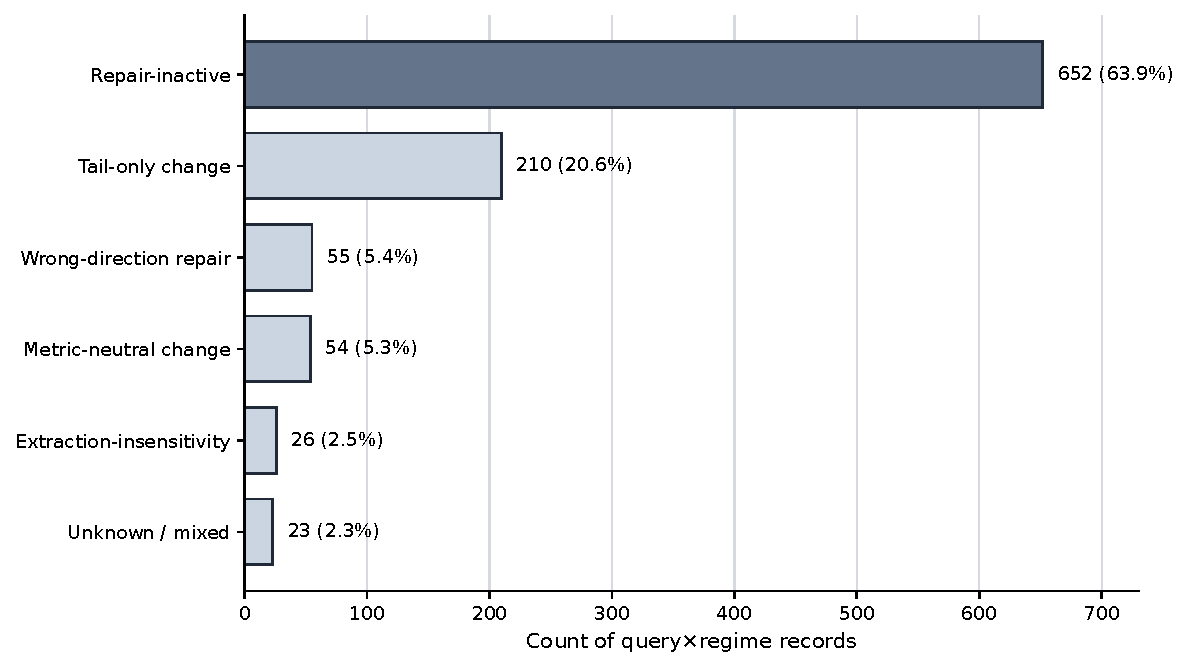
\includegraphics[width=0.98\linewidth]{../../../figures/manuscript/fig_failure_classes.pdf}
  \caption{Distribution of manual failure classes across 1,020
    query$\times$regime records. Repair-inactive (63.9\%) and tail-only
    change (20.6\%) account for the large majority of cases and describe
    mechanisms by which a structural repair fails to reach the retrieval
    metric at all, rather than mechanisms of active harm. Wrong-direction
    repair (5.4\%) is the only class with a materially negative mean
    $\Delta$nDCG and represents the minority of cases in which repair is
    actively unhelpful. See Table~\ref{tab:failure-taxonomy} for exact
    counts, percentages, and mean $\Delta$nDCG per class.}
  \Description{Horizontal bar chart of six manual failure classes ordered by
    count: Repair-inactive 652 (63.9 percent), Tail-only change 210
    (20.6 percent), Wrong-direction repair 55 (5.4 percent), Metric-neutral
    change 54 (5.3 percent), Extraction-insensitivity 26 (2.5 percent), and
    Unknown or mixed 23 (2.3 percent).}
  \label{fig:failure-classes}
\end{figure}

Two mechanisms recur across these classes and connect back to earlier
sections. First, candidate ordering and graph construction jointly determine
whether repair has anything to act on: Section~\ref{sec:structural-results}
showed this at the graph level (cyclicity by regime), and the
repair-inactive class shows it at the query level. Second, fusion can
suppress a graph-level change from ever reaching the final ranking: for the
Copeland component under the reciprocal-rank-fusion combination used in the
main hybrid ($\alpha = 0.3$), a repair-induced change to the raw graph
ranking is masked by fusion --- the fused ranking is unchanged even though
the underlying graph ranking is not --- in 14.7\% of query-method comparisons
where the graph ranking changed at all (\texttt{extraction\_fusion\_complete.csv});
the corresponding rate varies by component and fusion mode, from 4.8\% to
26.4\%. This is a contributing mechanism for a subset of the null results
above, not a single explanation for all of them: it is consistent with, and
partially overlaps, the tail-only-change and extraction-insensitivity
classes, but the taxonomy's six categories should be read as the more
complete account.

The practical interpretation is direct: for a retrieval pipeline
considering whether to add graph repair, the taxonomy indicates that the
typical outcome is inactivity or an invisible tail-only change, a small
fraction of cases are neutral or actively harmful, and a reliable positive
effect is rare and regime-specific (Section~\ref{sec:downstream-results}).
This is a diagnostic account of \emph{why} repair behaves this way in the
cases observed, not a validated predictive rule for deciding in advance
whether a new query or dataset will fall into one class or another; we
return to this distinction in Section~\ref{sec:discussion}.

\FloatBarrier

% =============================================================================
\section{Bounded Real-LLM Validation}
\label{sec:real-llm}

The main evidence base (Sections~\ref{sec:structural-results}--\ref{sec:failure-taxonomy})
uses mechanical, score-derived votes from BM25, TF-IDF, and MiniLM
(Section~\ref{sec:rankers}). This section reports a bounded check of whether
the same regime-conditional pattern persists under genuine large-language-model
pairwise judgments. The paired summary in Table~\ref{tab:real-llm-summary}
uses OpenAI pairwise judgments on SciDocs, HotpotQA, and FiQA. Separately,
the repository contains a protocol-distinct multi-provider failure-mining
corpus with Cohere/Azure pairwise judgments on FiQA, HotpotQA, and BRIGHT;
because it compares repaired and unrepaired Markov rankings under a different
query sample and sampling design, we do not pool it with
Table~\ref{tab:real-llm-summary} or treat it as a direct replication.

\begin{table}[t]
  \caption{Real-LLM pairwise pilot summary. $\Delta$nDCG is repaired minus
    unrepaired Copeland hybrid. Source:
    \texttt{openai\_real\_llm\_cross\_dataset\_summary.md}.}
  \label{tab:real-llm-summary}
  \begin{tabular}{lccc}
    \toprule
    Dataset & Queries & Cyclic\% & $\Delta$nDCG (95\% CI) \\
    \midrule
    SciDocs  & 50 & 92.0 & $-0.0010$ $[-0.0019, -0.0002]$ \\
    HotpotQA & 20 & 80.0 & $0.0$ $[0, 0]$ \\
    FiQA     & 10\textsuperscript{a} & 10.0 & $0.0$ $[0, 0]$ \\
    \bottomrule
  \end{tabular}
  \\[2pt]
  \footnotesize\textsuperscript{a}10 of a 20-query target were successfully
  processed; the remaining 10 are not included in this summary.
\end{table}

Cyclicity under real LLM pairwise judgments is, as under the mechanical
votes, regime- and dataset-sensitive: SciDocs and HotpotQA form a
high-cyclicity setting (92.0\% and 80.0\% of queries), while FiQA is
low-cyclicity in this run (10.0\%). Repaired-versus-unrepaired Copeland
$\Delta$nDCG is small throughout: SciDocs shows a small \emph{negative}
effect with a 95\% CI that excludes zero ($-0.0010$, $[-0.0019, -0.0002]$);
HotpotQA and FiQA are both degenerate at exactly zero. We report the SciDocs
result plainly rather than softening it: the one real-LLM cell with a
confidently non-null effect in this study is negative, not positive,
reinforcing rather than contradicting the decoupling pattern of
Section~\ref{sec:downstream-results}.

The protocol-distinct multi-provider corpus is directionally consistent with
the same picture while broadening scope to BRIGHT and a second provider
family. Across its 200 query-regime records, repair is inactive in all
62 \texttt{ms2} records and all 69 \texttt{ms1\_drop\_mutual} records; in
\texttt{ms1}, it yields one help case and one harm case among 69 records.
Because that corpus compares repaired and unrepaired Markov rankings rather
than the Copeland-hybrid pair summarized in Table~\ref{tab:real-llm-summary},
we use it only as corroborative scope evidence rather than as a pooled
estimate.

This evidence is corroborative, not primary. Query budgets are small (10--50
per dataset, an order of magnitude or more below the mechanical-vote
package's per-regime counts in Table~\ref{tab:dataset-stats}), the paired
cross-dataset summary itself uses a single provider, and FiQA's count
reflects partial processing of a larger target. The separate multi-provider
corpus extends scope but follows a different protocol and method pair. We
treat this section as a bounded check that the
structural/retrieval decoupling pattern is not an artifact specific to
mechanical score-derived votes, not as an independent confirmation at the
same evidentiary standard as Sections~\ref{sec:structural-results}--\ref{sec:failure-taxonomy},
and we do not draw conclusions from it beyond that limited scope.

% =============================================================================
\section{Efficiency and Practical Considerations}
\label{sec:efficiency}

We summarize existing runtime and memory evidence from the real-data pipeline
(Section~\ref{sec:implementation}); this section reports only measurements
already collected, not a new benchmarking exercise. On the full evaluation
dataset, greedy repair's measured wall-clock cost is effectively at the
resolution floor of our timing instrumentation ($\approx 0$s per query in the
pooled aggregation); exact-for-small-components adds a modest, measurable
overhead (mean $0.062$s per query, mean peak RSS $\approx 1{,}646$MB) relative
to the same baseline. Given the retrieval-quality comparison in
Section~\ref{sec:downstream-results}, this additional cost buys no retrieval
benefit on this corpus: exact-for-small-components' pooled Copeland nDCG is
statistically indistinguishable from greedy's. The practical implication is
direct --- for the datasets and graph sizes studied here, greedy repair is
the more favorable operating point on cost alone, since the exact variant's
only measurable advantage (marginally more structural weight removed on some
queries) does not translate into a retrieval-quality difference large enough
to justify its overhead.

We are explicit about the limits of this evidence. Runtime and memory were
measured on a single, unbenchmarked local development machine
(Section~\ref{sec:implementation}), not a controlled hardware configuration,
so absolute figures should not be read as generalizing to other environments;
memory is a coarse before/after resident-set-size snapshot, not instrumented
peak-memory tracking. We are not aware of a publicly documented, comparable real-data
memory benchmark beyond the single comparison reported here, and we do not
extrapolate from it to a general efficiency claim. A separate, purely
synthetic runtime study elsewhere in the supporting materials (dense
synthetic graphs, up to 100 items) shows repair cost growing steeply with
graph size, but that study uses artificially dense graphs unlike the sparser
real preference graphs evaluated here, and we do not treat it as evidence
about the real pipeline's scaling behavior.

% =============================================================================
\section{CARB Benchmark}
\label{sec:carb}

Alongside the empirical findings above, we plan to release the
\emph{Consistency-Aware Reranking Benchmark} (CARB), a companion resource
that packages the graph-theoretic features, repair outcomes, ranking scores,
and diagnostic labels underlying Sections~\ref{sec:structural-results}--\ref{sec:failure-taxonomy}
for reuse in future preference-graph data-quality research. CARB is a
companion reproducibility and benchmarking resource to this paper's empirical
findings, not the paper's primary contribution.

The unit of observation is a (query, vote-extraction regime, method) triple.
Table~\ref{tab:carb-stats} summarizes the planned release's scope: 440
independent queries across the four datasets studied in this paper, 1,020
query$\times$regime records (Section~\ref{sec:regimes}), and up to 366
ranking-method outputs per record, organized into 14 or more feature groups
spanning pre-repair graph structure (cyclicity, SCC size, edge counts),
repair outcomes (FAS weight removed), ranking scores, and the failure-class
labels of Section~\ref{sec:failure-taxonomy}.

\begin{table}[t]
  \caption{Planned CARB release statistics.}
  \label{tab:carb-stats}
  \begin{tabular}{lc}
    \toprule
    Statistic & Value \\
    \midrule
    Independent queries        & 440 \\
    Query$\times$regime records & 1{,}020 \\
    Methods per record          & 366 \\
    Feature groups              & 14+ \\
    Source datasets             & SciDocs, FiQA, HotpotQA, BRIGHT \\
    \bottomrule
  \end{tabular}
\end{table}

Provenance is derived entirely from the four public source datasets already
cited (Section~\ref{sec:datasets}) and from the mechanical ranker scores and
repair pipeline described in Sections~\ref{sec:methodology}
and~\ref{sec:experimental-setup}; no raw document text or third-party corpus
content is intended for redistribution, and any redistribution is planned to
be feature-only (graph statistics, scores, and labels), respecting the
licensing terms of the underlying source datasets. We plan to accompany the
release with a data card documenting schema, provenance, known limitations
(including the BEW/PIC circularity noted in Section~\ref{sec:structural-results}
and the failure-label taxonomy's manual-review basis), and intended uses ---
principally, reproducible research on preference-graph structural data
quality and repair, not training data for a production ranking system. At the
time of writing, CARB's schema and feature dictionary have been specified but
the release itself has not been packaged or made public; we plan a versioned
public release (beginning at v0.1) via an archival and Hugging Face Datasets
Hub distribution once packaging is complete, timed to camera-ready
preparation, together with a stable citation for the resource itself. No
claim in this paper depends on CARB's public availability; it is offered as
a reproducibility and follow-on-research aid, not as a precondition for
verifying the results reported above.

% =============================================================================
\section{Discussion}
\label{sec:discussion}

The results assembled in Sections~\ref{sec:structural-results}--\ref{sec:efficiency}
support a single, consistent interpretation: structural consistency and
downstream retrieval utility are related but separable dimensions of data
quality, and improving the former is not a reliable route to improving the
latter. We discuss what this decoupling means, why it arises mechanically
rather than incidentally, and what would be required to move beyond a
diagnostic account toward a predictive one.

\textbf{Why repair can succeed mathematically but fail operationally.} FAS
repair (Eq.~\eqref{eq:mwfas}) is defined entirely in terms of the preference
graph's own edge weights; nothing in that objective references the relevance
judgments a retrieval metric is scored against. Section~\ref{sec:structural-results}
confirms repair does what it is designed to do --- reduce backward-edge
weight and pairwise inconsistency relative to a reference ranking --- exactly
when the graph is cyclic. But because the objective and the downstream metric
are formally independent, a repair step can succeed completely on its own
terms while being irrelevant, neutral, or actively unhelpful once fused into
a final ranking. The failure taxonomy (Section~\ref{sec:failure-taxonomy})
gives this abstract observation concrete mechanisms: inactivity when the
graph has little to repair, invisibility when the change falls below the
evaluation cutoff, insensitivity when the scoring rule does not register the
specific edges removed, and, in a minority of cases, active harm when the
removed edges happened to be aligned with relevance rather than against it.

\textbf{Construction and extraction, not repair alone, govern the outcome.}
A recurring theme across Sections~\ref{sec:structural-results}
and~\ref{sec:downstream-results} is that vote-extraction regime, not the
repair step, is the dominant determinant of whether repair has any work to
do at all (Table~\ref{tab:structural-results}), and that the choice of
extraction rule (Copeland vs.\ balance, Eqs.~\eqref{eq:copeland}
and~\eqref{eq:balance}) shapes whether a structural change reaches the final
score once it does occur --- the balance hybrid is uniformly repair-invariant
across every cell we test (Table~\ref{tab:bootstrap-delta-ndcg}), while
Copeland is not. Preference construction, graph repair, and ranking
extraction are three separable design choices with distinct empirical
consequences, and treating ``graph repair'' as a single monolithic
intervention obscures where its effects actually originate.

\textbf{Fusion is both a stabilizer and a suppressor.} The hybrid combination
(Eq.~\eqref{eq:hybrid}) mixes a graph-derived component into a prior ranking
at a fixed weight $\alpha$. This stabilizes the final ranking against noisy
or spurious graph-level changes --- a virtue when the graph signal is
unreliable --- but the same mechanism can suppress a genuine, repair-induced
structural change before it reaches the retrieval metric
(Section~\ref{sec:failure-taxonomy}, 14.7\% suppression rate for the main
hybrid's component/fusion combination). Which effect dominates is not
knowable from $\alpha$ alone; it depends on the interaction between how much
the graph changed and how the fusion weight discounts that change relative
to the prior, which is why we treat fusion suppression as a diagnostic
finding rather than a tunable knob to optimize in this study.

\textbf{Dataset-specific effects resist a simple structural explanation.}
HotpotQA is the one dataset with a retrieval effect distinguishable from
noise, and it is also the least cyclic of the four datasets under
\texttt{ms1} (Table~\ref{tab:structural-results}) --- the opposite of what a
naive ``more inconsistency, more room for repair to help'' account would
predict. We do not have a confirmed explanation for why HotpotQA behaves this
way; plausible candidates include its multi-hop structure interacting
differently with the three constituent rankers, or dataset-specific relevance
grading conventions, but distinguishing between these would require new
experiments outside this paper's scope. We flag this as the clearest
open question this study raises rather than resolves.

\textbf{Implications for preference-graph ranking research.} Taken together,
these findings suggest that future work in this area should report structural
and retrieval outcomes separately by default, rather than assuming the former
predicts the latter, and should treat vote construction as a first-class
experimental factor rather than fixed preprocessing. Stronger optimization of
the structural objective alone is not sufficient to change this picture:
Section~\ref{sec:downstream-results}'s exact-for-small-components comparison
shows that solving the same objective more thoroughly than a greedy heuristic
does not translate into a retrieval-quality gain, because the objective being
optimized more thoroughly is still not the metric ultimately being evaluated.
A genuinely predictive criterion for \emph{when} repair will help --- as
opposed to the retrospective taxonomy offered here --- would need to identify,
in advance of running repair, some observable property of a query's graph or
candidate set that correlates with which failure class it will fall into;
our exploratory attempts in this direction do not produce such a rule.
Learned logistic and shallow-tree selectors do not beat a simple
disagreement-threshold policy overall, and failure-pattern classifiers reach
ROC-AUC in the mid-0.8s but only modest precision-recall on these rare
positive cases. We therefore do not claim a validated predictive criterion.

\textbf{Answering the original question.} We set out to ask when repairing
preference-graph inconsistency improves downstream retrieval quality. The
answer supported by this study is: rarely, and only when the vote-extraction
regime has already made the graph substantially cyclic, and even then in a
dataset-dependent way that is not explained by cyclicity severity alone. The
more actionable finding is the negative one --- knowing when repair is
inactive, invisible, or neutral is itself useful guidance for a practitioner
deciding whether to add a repair step to a retrieval pipeline, since it
identifies the large majority of cases in which the intervention would be
pure overhead.

% =============================================================================
\section{Limitations}
\label{sec:threats}

We state the limitations of this study candidly, several of which have
already been flagged at first relevance earlier in the paper rather than
held back for this section alone.

\textbf{Real-LLM scale.} Section~\ref{sec:real-llm}'s paired cross-dataset
pilot uses 10--50 queries per dataset and a single provider. The repository
also contains a separate 200-record multi-provider failure-mining corpus with
Cohere/Azure judgments and BRIGHT coverage, but that corpus uses a different
method pair, query sample, and protocol. Together these streams are
sufficient to show that the main decoupling pattern is not obviously confined
to one provider or to the mechanical-vote setting, but not sufficient to
establish how it behaves under LLM judgments in general.

\textbf{No validated predictive selector.} The failure taxonomy
(Section~\ref{sec:failure-taxonomy}) explains, retrospectively, why repair
succeeded or failed in the cases observed. It is not a validated criterion
for predicting, in advance, whether repair will help on a new query or
dataset; exploratory learned selectors do not beat a fixed disagreement
threshold overall, and failure-pattern models show limited precision-recall
on rare positive cases (Section~\ref{sec:discussion}). We do not claim
otherwise.

\textbf{Protocol differences across experiment families.} The vote-extraction
suite (Sections~\ref{sec:structural-results}--\ref{sec:downstream-results},
first two subsections) and the pooled failure-mining corpus
(Section~\ref{sec:downstream-results}'s baseline comparison,
Section~\ref{sec:failure-taxonomy}) share method implementations but not
query populations; we have flagged this distinction at each point it matters
(Section~\ref{sec:baselines}), but a reader assembling numbers across
sections should not treat the two corpora as interchangeable.

\textbf{HotpotQA sample size.} HotpotQA's \texttt{ms1} cell --- the one
regime with a retrieval effect distinguishable from noise --- has $n=52$
queries, smaller than SciDocs or FiQA's corresponding cells. The bootstrap CI
we report (Table~\ref{tab:bootstrap-delta-ndcg}) already reflects this
sample size, but a result resting on 52 queries warrants caution before
generalizing beyond this study.

\textbf{Structural metrics tied to the repair objective.} BEW and PIC
(Section~\ref{sec:structural-results}) are computed against a reference
ranking derived from the same relevance judgments used for downstream nDCG
evaluation. This is a qrels-anchored structural diagnostic, not an
independent measure of graph correctness, and should not be read as
external validation that repair improves some ground truth beyond the
evaluation data itself.

\textbf{Incomplete memory benchmarking.} As stated in
Section~\ref{sec:efficiency}, memory measurements are a coarse before/after
snapshot on a single, unbenchmarked machine, and we are not aware of a
documented real-data memory benchmark beyond the one comparison reported. We
do not make a general efficiency claim beyond that bounded evidence.

\textbf{Bounded exact-solver coverage.} The stronger-repair comparison
(Section~\ref{sec:downstream-results}) that is fully reproducible from this
repository covers the complete evaluation dataset, but the additional
robustness check against further exact and metaheuristic solvers
(Section~\ref{sec:repair-variants}) covers only a fixed sample of cyclic
queries using a separate package withheld from citation during review; we
do not treat that additional check as full-coverage evidence.

\textbf{Derived-data licensing constraints.} The planned CARB release
(Section~\ref{sec:carb}) is restricted to feature-only redistribution,
respecting the source datasets' own licensing terms; it is not a
redistribution of raw document text, and any use of CARB remains subject to
the original datasets' licenses for the underlying corpora.

\textbf{No claim of universal external validity.} The central findings
summarized in Section~\ref{sec:discussion} are established on four datasets,
three vote-extraction regimes, and a three-ranker mechanical voting scheme
(BM25, TF-IDF, MiniLM). We do not claim these findings generalize to
arbitrarily different ranker families, domains, or preference-construction
procedures beyond what Section~\ref{sec:real-llm}'s bounded check already
covers.

% =============================================================================
\section{Conclusion}
\label{sec:conclusion}

This paper studied preference-graph inconsistency as a measurable structural
data-quality dimension and evaluated feedback-arc-set repair as a candidate
improvement technique, across four public retrieval benchmarks and three
vote-extraction regimes. Repair reliably improves structural consistency
(reduced backward-edge weight and pairwise inconsistency) whenever the
underlying graph is substantially cyclic, and vote-extraction regime, not
repair itself, is the dominant determinant of whether that condition holds
at all. That structural improvement, however, does not reliably translate
into a downstream retrieval-quality gain: twenty of twenty-four
dataset-regime-method cells show no retrieval effect whatsoever, and among
the four cells where the graph is substantially cyclic, only one --- HotpotQA
under the most permissive vote-extraction regime --- shows an effect
distinguishable from noise, and that effect is not explained by cyclicity
severity alone. Strong, simple aggregation baselines that never inspect
graph structure at all, CombSUM and reciprocal rank fusion in particular,
remain competitive with or superior to every graph-based method evaluated,
including repaired hybrids. A six-class manual failure taxonomy indicates
that the typical outcome of applying repair is inactivity or an evaluation-
invisible tail change, that active harm is a small minority of cases, and
that a reliable positive effect is rare and regime-specific. These findings
were corroborated, within a bounded scope, by an OpenAI pairwise pilot on
SciDocs, HotpotQA, and FiQA and by a separate protocol-distinct
Cohere/Azure failure-mining corpus that includes BRIGHT. Alongside these findings,
we plan to release CARB, a companion benchmark resource packaging the
graph features, repair outcomes, and diagnostic labels underlying this
study, to support reproducible follow-on research on preference-graph data
quality. The practical takeaway is deliberately modest rather than
promotional: a practitioner deciding whether to add graph repair to a
retrieval pipeline should expect it to succeed as a structural intervention
far more often than as a retrieval-quality one, and should budget for that
distinction rather than assume the two travel together.

% =============================================================================
\section{Data Availability and Reproducibility}
\label{sec:data-availability}

\textbf{Data availability.} All four source datasets (SciDocs, FiQA,
HotpotQA, BRIGHT) are publicly available from their original
sources~\cite{cohan2020scidocs,maia2018fiqa,yang2018hotpotqa,su2024bright}
under their respective licenses; this paper introduces no new raw-text
corpus. The derived preference-graph features, repair outcomes, and
diagnostic labels underlying Sections~\ref{sec:structural-results}--\ref{sec:failure-taxonomy}
are planned for release as the CARB companion resource
(Section~\ref{sec:carb}), feature-only and license-compatible with the
source datasets; that release is not yet public as of this draft.

\textbf{Artifact availability.} The full pipeline (vote extraction, graph
construction, repair, ranking extraction, evaluation, and bootstrap analysis;
Sections~\ref{sec:methodology}--\ref{sec:experimental-setup}) is implemented
in a single code repository. For double-blind review, the repository
identity and URL are withheld; an anonymized or author-provided artifact
will be made available to reviewers upon request through the venue's
standard mechanism, and the repository will be made public upon acceptance.

\textbf{Reproducibility.} Every table in Sections~\ref{sec:structural-results}--\ref{sec:downstream-results}
is generated from versioned, released intermediate outputs by scripted,
deterministic aggregation; the vote-extraction protocol
(Section~\ref{sec:vote-extraction}), regime definitions
(Section~\ref{sec:regimes}), and bootstrap procedure
(Section~\ref{sec:bootstrap}) are fully specified with fixed parameters
(thresholds, $\alpha$, $B=2{,}000$ resamples) so that all reported means and
confidence intervals can be regenerated from the same released inputs
without repeating the original API-free, CPU-only computation. The one
exception is the bounded robustness check against additional exact and
metaheuristic solvers (Section~\ref{sec:repair-variants}), which depends on
a separate package withheld from citation during review and is reported
qualitatively rather than as a table for this reason; full reproduction
details for that check will accompany the camera-ready version.

\begin{acks}
% TODO(manuscript-authors): omit or anonymize for double-blind review; restore
% on camera-ready only. Do not include funding/acknowledgment text that could
% deanonymize authorship before that point.
\end{acks}

\bibliographystyle{ACM-Reference-Format}
\bibliography{references}

\end{document}
